% Options for packages loaded elsewhere
% Options for packages loaded elsewhere
\PassOptionsToPackage{unicode}{hyperref}
\PassOptionsToPackage{hyphens}{url}
\PassOptionsToPackage{dvipsnames,svgnames,x11names}{xcolor}
%
\documentclass[
  french,
  10pt,
  a4paper,
]{article}
\usepackage{xcolor}
\usepackage[top=20mm,left=20mm,right=20mm,bottom=20mm]{geometry}
\usepackage{amsmath,amssymb}
\setcounter{secnumdepth}{5}
\usepackage{iftex}
\ifPDFTeX
  \usepackage[T1]{fontenc}
  \usepackage[utf8]{inputenc}
  \usepackage{textcomp} % provide euro and other symbols
\else % if luatex or xetex
  \usepackage{unicode-math} % this also loads fontspec
  \defaultfontfeatures{Scale=MatchLowercase}
  \defaultfontfeatures[\rmfamily]{Ligatures=TeX,Scale=1}
\fi
\usepackage{lmodern}
\ifPDFTeX\else
  % xetex/luatex font selection
  \setmainfont[]{Raleway}
  \setsansfont[]{Avenir Next LT Pro}
  \setmonofont[Scale=0.9]{Consolas}
\fi
% Use upquote if available, for straight quotes in verbatim environments
\IfFileExists{upquote.sty}{\usepackage{upquote}}{}
\IfFileExists{microtype.sty}{% use microtype if available
  \usepackage[]{microtype}
  \UseMicrotypeSet[protrusion]{basicmath} % disable protrusion for tt fonts
}{}
\makeatletter
\@ifundefined{KOMAClassName}{% if non-KOMA class
  \IfFileExists{parskip.sty}{%
    \usepackage{parskip}
  }{% else
    \setlength{\parindent}{0pt}
    \setlength{\parskip}{6pt plus 2pt minus 1pt}}
}{% if KOMA class
  \KOMAoptions{parskip=half}}
\makeatother
% Make \paragraph and \subparagraph free-standing
\makeatletter
\ifx\paragraph\undefined\else
  \let\oldparagraph\paragraph
  \renewcommand{\paragraph}{
    \@ifstar
      \xxxParagraphStar
      \xxxParagraphNoStar
  }
  \newcommand{\xxxParagraphStar}[1]{\oldparagraph*{#1}\mbox{}}
  \newcommand{\xxxParagraphNoStar}[1]{\oldparagraph{#1}\mbox{}}
\fi
\ifx\subparagraph\undefined\else
  \let\oldsubparagraph\subparagraph
  \renewcommand{\subparagraph}{
    \@ifstar
      \xxxSubParagraphStar
      \xxxSubParagraphNoStar
  }
  \newcommand{\xxxSubParagraphStar}[1]{\oldsubparagraph*{#1}\mbox{}}
  \newcommand{\xxxSubParagraphNoStar}[1]{\oldsubparagraph{#1}\mbox{}}
\fi
\makeatother

\usepackage{color}
\usepackage{fancyvrb}
\newcommand{\VerbBar}{|}
\newcommand{\VERB}{\Verb[commandchars=\\\{\}]}
\DefineVerbatimEnvironment{Highlighting}{Verbatim}{commandchars=\\\{\}}
% Add ',fontsize=\small' for more characters per line
\newenvironment{Shaded}{}{}
\newcommand{\AlertTok}[1]{\textcolor[rgb]{0.58,0.85,0.30}{\textbf{\colorbox[rgb]{0.30,0.12,0.14}{#1}}}}
\newcommand{\AnnotationTok}[1]{\textcolor[rgb]{0.31,0.63,0.31}{#1}}
\newcommand{\AttributeTok}[1]{\textcolor[rgb]{0.65,0.15,0.64}{#1}}
\newcommand{\BaseNTok}[1]{\textcolor[rgb]{0.60,0.41,0.00}{#1}}
\newcommand{\BuiltInTok}[1]{\textcolor[rgb]{0.65,0.15,0.64}{#1}}
\newcommand{\CharTok}[1]{\textcolor[rgb]{0.31,0.63,0.31}{#1}}
\newcommand{\CommentTok}[1]{\textcolor[rgb]{0.63,0.63,0.65}{\textit{#1}}}
\newcommand{\CommentVarTok}[1]{\textcolor[rgb]{0.89,0.34,0.29}{\textit{#1}}}
\newcommand{\ConstantTok}[1]{\textcolor[rgb]{0.60,0.41,0.00}{#1}}
\newcommand{\ControlFlowTok}[1]{\textcolor[rgb]{0.65,0.15,0.64}{#1}}
\newcommand{\DataTypeTok}[1]{\textcolor[rgb]{0.65,0.15,0.64}{#1}}
\newcommand{\DecValTok}[1]{\textcolor[rgb]{0.60,0.41,0.00}{#1}}
\newcommand{\DocumentationTok}[1]{\textcolor[rgb]{0.89,0.34,0.29}{#1}}
\newcommand{\ErrorTok}[1]{\textcolor[rgb]{0.96,0.28,0.28}{\underline{#1}}}
\newcommand{\ExtensionTok}[1]{\textcolor[rgb]{0.25,0.47,0.95}{\textbf{#1}}}
\newcommand{\FloatTok}[1]{\textcolor[rgb]{0.60,0.41,0.00}{#1}}
\newcommand{\FunctionTok}[1]{\textcolor[rgb]{0.25,0.47,0.95}{#1}}
\newcommand{\ImportTok}[1]{\textcolor[rgb]{0.31,0.63,0.31}{#1}}
\newcommand{\InformationTok}[1]{\textcolor[rgb]{0.77,0.36,0.00}{#1}}
\newcommand{\KeywordTok}[1]{\textcolor[rgb]{0.65,0.15,0.64}{#1}}
\newcommand{\NormalTok}[1]{\textcolor[rgb]{0.22,0.23,0.26}{#1}}
\newcommand{\OperatorTok}[1]{\textcolor[rgb]{0.65,0.15,0.64}{#1}}
\newcommand{\OtherTok}[1]{\textcolor[rgb]{0.15,0.68,0.38}{#1}}
\newcommand{\PreprocessorTok}[1]{\textcolor[rgb]{0.65,0.15,0.64}{#1}}
\newcommand{\RegionMarkerTok}[1]{\textcolor[rgb]{0.16,0.50,0.73}{\colorbox[rgb]{0.08,0.19,0.26}{#1}}}
\newcommand{\SpecialCharTok}[1]{\textcolor[rgb]{0.00,0.52,0.74}{#1}}
\newcommand{\SpecialStringTok}[1]{\textcolor[rgb]{0.85,0.27,0.33}{#1}}
\newcommand{\StringTok}[1]{\textcolor[rgb]{0.31,0.63,0.31}{#1}}
\newcommand{\VariableTok}[1]{\textcolor[rgb]{0.89,0.34,0.29}{#1}}
\newcommand{\VerbatimStringTok}[1]{\textcolor[rgb]{0.85,0.27,0.33}{#1}}
\newcommand{\WarningTok}[1]{\textcolor[rgb]{0.85,0.27,0.33}{#1}}

\usepackage{longtable,booktabs,array}
\newcounter{none} % for unnumbered tables
\usepackage{calc} % for calculating minipage widths
% Correct order of tables after \paragraph or \subparagraph
\usepackage{etoolbox}
\makeatletter
\patchcmd\longtable{\par}{\if@noskipsec\mbox{}\fi\par}{}{}
\makeatother
% Allow footnotes in longtable head/foot
\IfFileExists{footnotehyper.sty}{\usepackage{footnotehyper}}{\usepackage{footnote}}
\makesavenoteenv{longtable}
\usepackage{graphicx}
\makeatletter
\newsavebox\pandoc@box
\newcommand*\pandocbounded[1]{% scales image to fit in text height/width
  \sbox\pandoc@box{#1}%
  \Gscale@div\@tempa{\textheight}{\dimexpr\ht\pandoc@box+\dp\pandoc@box\relax}%
  \Gscale@div\@tempb{\linewidth}{\wd\pandoc@box}%
  \ifdim\@tempb\p@<\@tempa\p@\let\@tempa\@tempb\fi% select the smaller of both
  \ifdim\@tempa\p@<\p@\scalebox{\@tempa}{\usebox\pandoc@box}%
  \else\usebox{\pandoc@box}%
  \fi%
}
% Set default figure placement to htbp
\def\fps@figure{htbp}
\makeatother



\ifLuaTeX
\usepackage[bidi=basic,shorthands=off]{babel}
\else
\usepackage[bidi=default,shorthands=off]{babel}
\fi
\ifPDFTeX
\else
\babelfont{rm}[]{Raleway}
\fi
\ifLuaTeX
  \usepackage{selnolig} % disable illegal ligatures
\fi


\setlength{\emergencystretch}{3em} % prevent overfull lines

\providecommand{\tightlist}{%
  \setlength{\itemsep}{0pt}\setlength{\parskip}{0pt}}



 


\usepackage{booktabs}
\usepackage{longtable}
\usepackage{array}
\usepackage{multirow}
\usepackage{wrapfig}
\usepackage{float}
\usepackage{colortbl}
\usepackage{pdflscape}
\usepackage{tabularx}
\usepackage{xltabular}
\usepackage{threeparttable}
\usepackage{threeparttablex}
\usepackage[normalem]{ulem}
\usepackage{makecell}
\usepackage{xcolor}
\usepackage{graphicx} % pour insérer des images
\usepackage{fancyhdr} % gestion du header / footer
\pagestyle{plain}     % style par défaut avec numéro de page centré en bas

% STYLE « firstpage » : pied de page personnalisé pour la première page
\fancypagestyle{firstpage}{
  % vide header et footer
  \fancyhf{} % 
  % --- suppression des lignes horizontales ---
  \renewcommand{\headrulewidth}{0pt} % supprime la ligne horizontale de l'en-tête
  \renewcommand{\footrulewidth}{0pt} % supprime la ligne horizontale du pied de page
  % --- ajustement local de la distance du bas = augmenter \footskip localement avec \setlength ---
  \setlength{\footskip}{1pt}
  %  --- contenu du pied de page centré ---
  \fancyfoot[C]{%
    Diffusé sous licence~%
    \href{https://creativecommons.org/licenses/by-nc-sa/4.0/}{%
    \textbf{CC BY‑NC‑SA 4.0}%
    } \\[6pt] % texte avec saut de ligne vertical
    
\includegraphics[height=1cm]{img/Licence_cc-by-nc-sa.png} \\[10pt] % logo en dessous puis ligne vide supplémentaire
    }
    }
\makeatletter
\@ifpackageloaded{tcolorbox}{}{\usepackage[skins,breakable]{tcolorbox}}
\@ifpackageloaded{fontawesome5}{}{\usepackage{fontawesome5}}
\definecolor{quarto-callout-color}{HTML}{909090}
\definecolor{quarto-callout-note-color}{HTML}{0758E5}
\definecolor{quarto-callout-important-color}{HTML}{CC1914}
\definecolor{quarto-callout-warning-color}{HTML}{EB9113}
\definecolor{quarto-callout-tip-color}{HTML}{00A047}
\definecolor{quarto-callout-caution-color}{HTML}{FC5300}
\definecolor{quarto-callout-color-frame}{HTML}{acacac}
\definecolor{quarto-callout-note-color-frame}{HTML}{4582ec}
\definecolor{quarto-callout-important-color-frame}{HTML}{d9534f}
\definecolor{quarto-callout-warning-color-frame}{HTML}{f0ad4e}
\definecolor{quarto-callout-tip-color-frame}{HTML}{02b875}
\definecolor{quarto-callout-caution-color-frame}{HTML}{fd7e14}
\makeatother
\makeatletter
\@ifpackageloaded{caption}{}{\usepackage{caption}}
\AtBeginDocument{%
\ifdefined\contentsname
  \renewcommand*\contentsname{Table des matières}
\else
  \newcommand\contentsname{Table des matières}
\fi
\ifdefined\listfigurename
  \renewcommand*\listfigurename{Liste des Figures}
\else
  \newcommand\listfigurename{Liste des Figures}
\fi
\ifdefined\listtablename
  \renewcommand*\listtablename{Liste des Tables}
\else
  \newcommand\listtablename{Liste des Tables}
\fi
\ifdefined\figurename
  \renewcommand*\figurename{Figure}
\else
  \newcommand\figurename{Figure}
\fi
\ifdefined\tablename
  \renewcommand*\tablename{Tableau}
\else
  \newcommand\tablename{Tableau}
\fi
}
\@ifpackageloaded{float}{}{\usepackage{float}}
\floatstyle{ruled}
\@ifundefined{c@chapter}{\newfloat{codelisting}{h}{lop}}{\newfloat{codelisting}{h}{lop}[chapter]}
\floatname{codelisting}{Listing}
\newcommand*\listoflistings{\listof{codelisting}{Liste des Listings}}
\captionsetup{labelsep=period}
\makeatother
\makeatletter
\makeatother
\makeatletter
\@ifpackageloaded{caption}{}{\usepackage{caption}}
\@ifpackageloaded{subcaption}{}{\usepackage{subcaption}}
\makeatother
\makeatletter
\@ifpackageloaded{tcolorbox}{}{\usepackage[skins,breakable]{tcolorbox}}
\makeatother
\makeatletter
\@ifundefined{shadecolor}{\definecolor{shadecolor}{rgb}{.97, .97, .97}}{}
\makeatother
\makeatletter
\makeatother
\makeatletter
\ifdefined\Shaded\renewenvironment{Shaded}{\begin{tcolorbox}[borderline west={3pt}{0pt}{shadecolor}, boxrule=0pt, breakable, enhanced, frame hidden, interior hidden, sharp corners]}{\end{tcolorbox}}\fi
\makeatother
\usepackage{bookmark}
\IfFileExists{xurl.sty}{\usepackage{xurl}}{} % add URL line breaks if available
\urlstyle{same}
% fallback for those not using the hyperref driver hyperxmp:
\makeatletter
\@ifundefined{xmpquote}{\newcommand{\xmpquote}[1]{#1}}{}
\makeatother
\hypersetup{
  pdftitle={Bulle d'R. (Re)Découvrir R et RStudio},
  pdfauthor={Sandrine LYSER},
  pdflang={fr},
  colorlinks=true,
  linkcolor={blue},
  filecolor={Maroon},
  citecolor={Blue},
  urlcolor={Blue},
  pdfcreator={LaTeX via pandoc}}


\title{Bulle d'R. (Re)Découvrir R et RStudio}
\author{Sandrine LYSER}
\date{22 septembre 2026}
\begin{document}
\maketitle

\renewcommand*\contentsname{Table des matières}
{
\setcounter{tocdepth}{3}
\tableofcontents
}

\thispagestyle{firstpage}
\pagebreak

\section{Préambule}\label{pruxe9ambule}

\subsection*{\texorpdfstring{\protect
\includegraphics[width=1em,height=1em]{index_files/figure-pdf/fa-icon-1844f4b8d02fb562f763d29311285e52.pdf}
Jeu de données utilisé dans cette
session}{ Jeu de données utilisé dans cette session}}\label{jeu-de-donnuxe9es-utilisuxe9-dans-cette-session}

Les exemples s'appuient sur le jeu de données \texttt{Journals},
disponible dans le package \{Ecdat\}

Ce jeu de données se compose de 180 observations décrites par 10
variables

\begin{itemize}
\tightlist
\item
  \textbf{title} : titre de la revue
\item
  \textbf{pub} : éditeur
\item
  \textbf{society} : société
\item
  \textbf{libprice} : prix de l'abonnement
\item
  \textbf{pages} : nombre de pages
\item
  \textbf{charpp} : nombre de caractères par page
\item
  \textbf{citestot} : nombre total de citations
\item
  \textbf{date1} : année de création de la revue
\item
  \textbf{oclc} : nombre d'abonnements
\item
  \textbf{field} : domaine de la revue
\end{itemize}

\section{Présentation des logiciels R et
RStudio}\label{pruxe9sentation-des-logiciels-r-et-rstudio}

\subsection{\texorpdfstring{\textbf{R} \emph{vs}
\textbf{RStudio}}{R vs RStudio}}\label{r-vs-rstudio}

\subsubsection{\texorpdfstring{\protect
\includegraphics[width=0.08\linewidth,height=\textheight,keepaspectratio]{img/Rlogo.png}}{}}\label{section}

\textbf{Langage de programmation} et \textbf{logiciel libre} pour la
statistique, la science des données et la visualisation, développé
depuis 1993

\begin{itemize}
\tightlist
\item
  Il ne s'agit pas d'un logiciel ``statique'' que l'on installe une fois
  pour des années, c'est tout un écosystème en \textbf{perpétuelle
  évolution, constamment mis à jour et amélioré}
\item
  C'est un logiciel libre distribué selon les termes de la licence GNU
  GPL (\emph{open source}), qui bénéficie d'une large communauté
  internationale et qui offre une multitude de fonctionnalités grâce aux
  packages
\item
  Compatible avec la plupart des systèmes d'exploitation (Windows,
  MacOS, Linux)
\item
  Disponible en téléchargement sur le site du
  \href{http://cran.r-project.org}{CRAN} (\emph{Comprehensive R Archive
  Network})
\end{itemize}

\begin{tcolorbox}[enhanced jigsaw, arc=.35mm, bottomrule=.15mm, breakable, colback=white, colframe=quarto-callout-note-color-frame, left=2mm, leftrule=.75mm, opacityback=0, rightrule=.15mm, toprule=.15mm]
\begin{minipage}[t]{5.5mm}
\textcolor{quarto-callout-note-color}{\faInfo}
\end{minipage}%
\begin{minipage}[t]{\textwidth - 5.5mm}

Dernière version disponible au 21 sept. 2026 : R version 4.6.1
(2026-06-24 ucrt) -- ``Happy Hop''

\emph{Cette session utilise R version 4.6.0 (2026-04-24 ucrt) --
``Because it was There''}

\end{minipage}%
\end{tcolorbox}

\begin{center}\rule{0.5\linewidth}{0.5pt}\end{center}

\paragraph{Les objets}\label{les-objets}

La programmation dans \textbf{R} repose sur des \textbf{objets}, qui
apparaîtront dans la fenêtre \emph{Environment} de \textbf{RStudio}\\
\(\Rightarrow\) \textbf{Dans R, presque tout est un objet : nombres,
textes, tableaux, graphiques, modèles, fonctions\ldots{}}

\begin{itemize}
\tightlist
\item
  Un objet est une structure de données avec

  \begin{itemize}
  \tightlist
  \item
    un nom (\emph{exemple} : x, donnees, modele)
  \item
    un contenu (une ou plusieurs valeurs)
  \item
    un type / mode (\emph{numeric}, \emph{character}, \emph{logical},
    etc.)
  \item
    parfois une classe (\emph{vector}, \emph{matrix}, \emph{data.frame},
    \emph{lm}, \emph{ggplot}, etc.)
  \end{itemize}
\item
  On crée un objet avec l'opérateur d'affectation noté
  \texttt{\textless{}-}, de la façon suivante :
  \texttt{nom\_objet\ \textless{}-\ valeur}\\
  \emph{Exemples}
\end{itemize}

\begin{Shaded}
\begin{Highlighting}[]
\NormalTok{x }\OtherTok{\textless{}{-}} \DecValTok{3}
\NormalTok{nom }\OtherTok{\textless{}{-}} \StringTok{"Alice"}
\NormalTok{df }\OtherTok{\textless{}{-}} \FunctionTok{data.frame}\NormalTok{(}\AttributeTok{age =} \FunctionTok{c}\NormalTok{(}\DecValTok{20}\NormalTok{, }\DecValTok{25}\NormalTok{), }\AttributeTok{sexe =} \FunctionTok{c}\NormalTok{(}\StringTok{"F"}\NormalTok{, }\StringTok{"H"}\NormalTok{))}
\end{Highlighting}
\end{Shaded}

\begin{tcolorbox}[enhanced jigsaw, arc=.35mm, bottomrule=.15mm, bottomtitle=1mm, breakable, colback=white, colbacktitle=quarto-callout-note-color!10!white, colframe=quarto-callout-note-color-frame, coltitle=black, left=2mm, leftrule=.75mm, opacityback=0, opacitybacktitle=0.6, rightrule=.15mm, title=\textcolor{quarto-callout-note-color}{\faInfo}\hspace{0.5em}{Note}, titlerule=0mm, toprule=.15mm, toptitle=1mm]

\begin{itemize}
\tightlist
\item
  S'il n'existe aucun objet qui porte le nom \texttt{nom\_objet} dans
  votre environnement de travail \textbf{R}, l'exécution de la commande
  crée un nouvel objet
\item
  S'il existe déjà un objet avec le nom \texttt{nom\_objet}, l'exécution
  de la commande écrase/met à jour l'ancien objet avec la nouvelle
  valeur
\end{itemize}

\end{tcolorbox}

\begin{center}\rule{0.5\linewidth}{0.5pt}\end{center}

\subparagraph{À quoi servent les objets
?}\label{uxe0-quoi-servent-les-objets}

\begin{itemize}
\tightlist
\item
  À stocker des données (vecteurs de mesures, colonnes d'un tableau,
  etc.) et des résultats (moyennes, modèles statistiques, tests,
  prédictions, etc.)
\item
  À structurer l'information : organiser les données en tableaux
  (\emph{dataframes}/\emph{tibbles}), listes, matrices, etc.
\item
  À réutiliser du code : les fonctions, graphiques, modèles sont
  eux-mêmes des objets \textbf{R} \(\Rightarrow\) En pratique, presque
  toutes les commandes \textbf{R} créent ou manipulent des objets
\end{itemize}

\begin{tcolorbox}[enhanced jigsaw, arc=.35mm, bottomrule=.15mm, bottomtitle=1mm, breakable, colback=white, colbacktitle=quarto-callout-tip-color!10!white, colframe=quarto-callout-tip-color-frame, coltitle=black, left=2mm, leftrule=.75mm, opacityback=0, opacitybacktitle=0.6, rightrule=.15mm, title=\textcolor{quarto-callout-tip-color}{\faLightbulb}\hspace{0.5em}{Comment nommmer les objets ?}, titlerule=0mm, toprule=.15mm, toptitle=1mm]

Vous pouvez donner n'importe quel nom à vos objets, en respectant
certaines règles

\begin{itemize}
\tightlist
\item
  le nom ne peut pas commencer par un chiffre
\item
  le nom ne doit pas contenir de caractères spéciaux (le
  \emph{underscore} \texttt{\_} est autorisé)
\item
  le nom ne doit pas être celui d'une fonction \textbf{R} déjà existante
  (\emph{exemple} : mean)
\end{itemize}

\end{tcolorbox}

\begin{center}\rule{0.5\linewidth}{0.5pt}\end{center}

\subparagraph{Les vecteurs}\label{les-vecteurs}

Le \textbf{vecteur} est le type d'objet de base, le plus simple\\
Il contient une ou plusieurs valeurs de même type

\begin{itemize}
\tightlist
\item
  du texte - \texttt{character} -
\item
  des nombres entiers - \texttt{integer} - ou réels - \texttt{double} ou
  \texttt{numeric} -
\item
  des valeurs logiques -\texttt{TRUE}(vrai) ou \texttt{FALSE}(faux) -
\end{itemize}

\emph{Exemples}

\begin{Shaded}
\begin{Highlighting}[]
\NormalTok{v\_log }\OtherTok{\textless{}{-}} \FunctionTok{c}\NormalTok{(}\ConstantTok{TRUE}\NormalTok{, }\ConstantTok{FALSE}\NormalTok{, }\ConstantTok{TRUE}\NormalTok{)}
\NormalTok{v\_num }\OtherTok{\textless{}{-}} \FunctionTok{c}\NormalTok{(}\FloatTok{1.5}\NormalTok{, }\FloatTok{2.7}\NormalTok{, }\FloatTok{3.0}\NormalTok{)}
\NormalTok{v\_txt }\OtherTok{\textless{}{-}} \FunctionTok{c}\NormalTok{(}\StringTok{"rouge"}\NormalTok{, }\StringTok{"vert"}\NormalTok{, }\StringTok{"bleu"}\NormalTok{)}
\end{Highlighting}
\end{Shaded}

\begin{center}\rule{0.5\linewidth}{0.5pt}\end{center}

\subparagraph{Les objets plus complexes
(1/2)}\label{les-objets-plus-complexes-12}

\begin{itemize}
\tightlist
\item
  Les \textbf{\emph{dataframes}} : des tableaux de données à 2
  dimensions, où les lignes sont les observations et les colonnes les
  variables \(\Rightarrow\) les colonnes peuvent avoir des types
  différents, mais ont toutes la même longueur
\end{itemize}


\includegraphics[width=0.75em,height=1em]{index_files/figure-pdf/fa-icon-04c6f9870c69c7270c705a206c46d917.pdf}
\textbf{Les données au format .csv ou .xls importées sous R sont des
\emph{dataframes}}

\emph{Exemple}

\begin{Shaded}
\begin{Highlighting}[]
\NormalTok{df }\OtherTok{\textless{}{-}} \FunctionTok{data.frame}\NormalTok{(}\AttributeTok{id   =} \DecValTok{1}\SpecialCharTok{:}\DecValTok{3}\NormalTok{,}
                 \AttributeTok{age  =} \FunctionTok{c}\NormalTok{(}\DecValTok{20}\NormalTok{, }\DecValTok{25}\NormalTok{, }\DecValTok{30}\NormalTok{),}
                 \AttributeTok{sexe =} \FunctionTok{c}\NormalTok{(}\StringTok{"F"}\NormalTok{, }\StringTok{"H"}\NormalTok{, }\StringTok{"H"}\NormalTok{),}
                 \AttributeTok{poids =} \FunctionTok{c}\NormalTok{(}\FloatTok{55.2}\NormalTok{, }\FloatTok{70.1}\NormalTok{, }\FloatTok{68.4}\NormalTok{))}
\end{Highlighting}
\end{Shaded}

\begin{itemize}
\tightlist
\item
  Les \textbf{matrices} : un objet à 2 dimensions (lignes × colonnes)
  qui contient des éléments du même type (des données numériques en
  général)
\end{itemize}

\emph{Exemple}

\begin{Shaded}
\begin{Highlighting}[]
\NormalTok{M }\OtherTok{\textless{}{-}} \FunctionTok{matrix}\NormalTok{(}\DecValTok{1}\SpecialCharTok{:}\DecValTok{6}\NormalTok{, }\AttributeTok{nrow =} \DecValTok{2}\NormalTok{, }\AttributeTok{ncol =} \DecValTok{3}\NormalTok{)}
\end{Highlighting}
\end{Shaded}

\begin{center}\rule{0.5\linewidth}{0.5pt}\end{center}

\subparagraph{Les objets plus complexes
(2/2)}\label{les-objets-plus-complexes-22}

\begin{itemize}
\tightlist
\item
  Les \textbf{listes} : une collection d'objets \textbf{R}, qui peuvent
  être de types différents \(\Rightarrow\) une liste peut contenir des
  vecteurs, des matrices, des \emph{dataframes}, d'autres listes, des
  fonctions, etc.
\end{itemize}

\emph{Exemple}

\begin{Shaded}
\begin{Highlighting}[]
\NormalTok{une\_liste }\OtherTok{\textless{}{-}} \FunctionTok{list}\NormalTok{(}\AttributeTok{age =} \FunctionTok{c}\NormalTok{(}\DecValTok{20}\NormalTok{, }\DecValTok{25}\NormalTok{, }\DecValTok{30}\NormalTok{),}
                  \AttributeTok{sexe =} \FunctionTok{c}\NormalTok{(}\StringTok{"F"}\NormalTok{, }\StringTok{"H"}\NormalTok{, }\StringTok{"H"}\NormalTok{),}
                  \AttributeTok{modele =} \FunctionTok{lm}\NormalTok{(poids }\SpecialCharTok{\textasciitilde{}}\NormalTok{ age, }\AttributeTok{data =}\NormalTok{ df))}
\end{Highlighting}
\end{Shaded}

\begin{itemize}
\tightlist
\item
  Les \textbf{facteurs} : un format spécial dans \textbf{R} pour les
  variables catégorielles (qualitatives), les modalités sont listées
  avec \texttt{levels} et peuvent être ordonnées (on parle alors
  d'\emph{ordered factor})
\end{itemize}

\emph{Exemple}

\begin{Shaded}
\begin{Highlighting}[]
\NormalTok{sexe }\OtherTok{\textless{}{-}} \FunctionTok{factor}\NormalTok{(}\FunctionTok{c}\NormalTok{(}\StringTok{"F"}\NormalTok{, }\StringTok{"H"}\NormalTok{, }\StringTok{"F"}\NormalTok{, }\StringTok{"H"}\NormalTok{), }
               \AttributeTok{levels =} \FunctionTok{c}\NormalTok{(}\StringTok{"F"}\NormalTok{, }\StringTok{"H"}\NormalTok{))}
\end{Highlighting}
\end{Shaded}

\subsubsection{\texorpdfstring{\protect
\includegraphics[width=0.15\linewidth,height=\textheight,keepaspectratio]{img/RStudiologo.png}}{}}\label{section-1}

\textbf{Environnement de développement intégré (IDE)} spécialement conçu
pour \textbf{R} avec une interface conviviale

\begin{itemize}
\tightlist
\item
  Logiciel \emph{open source}, gratuit et disponible pour la plupart des
  systèmes d'exploitation
\item
  Version locale (\emph{RStudio Desktop}) ou serveur (\emph{RStudio
  Server})
\item
  Quatre cadrants pour visualiser facilement les scripts, l'aide, les
  graphiques

  \begin{itemize}
  \tightlist
  \item
    \textbf{Source} (en haut à gauche) : éditeur de scripts
  \item
    \textbf{Environnement} (en haut à droite) : environnement de travail
    (objets, fonctions, etc.), historique, connexions, tutoriels
  \item
    \textbf{Console} (en bas à gauche) : exécution des commandes
  \item
    \textbf{Sorties} (en bas à droite) : fichiers, graphiques, packages,
    aide, visualiseur, présentation
  \end{itemize}
\end{itemize}

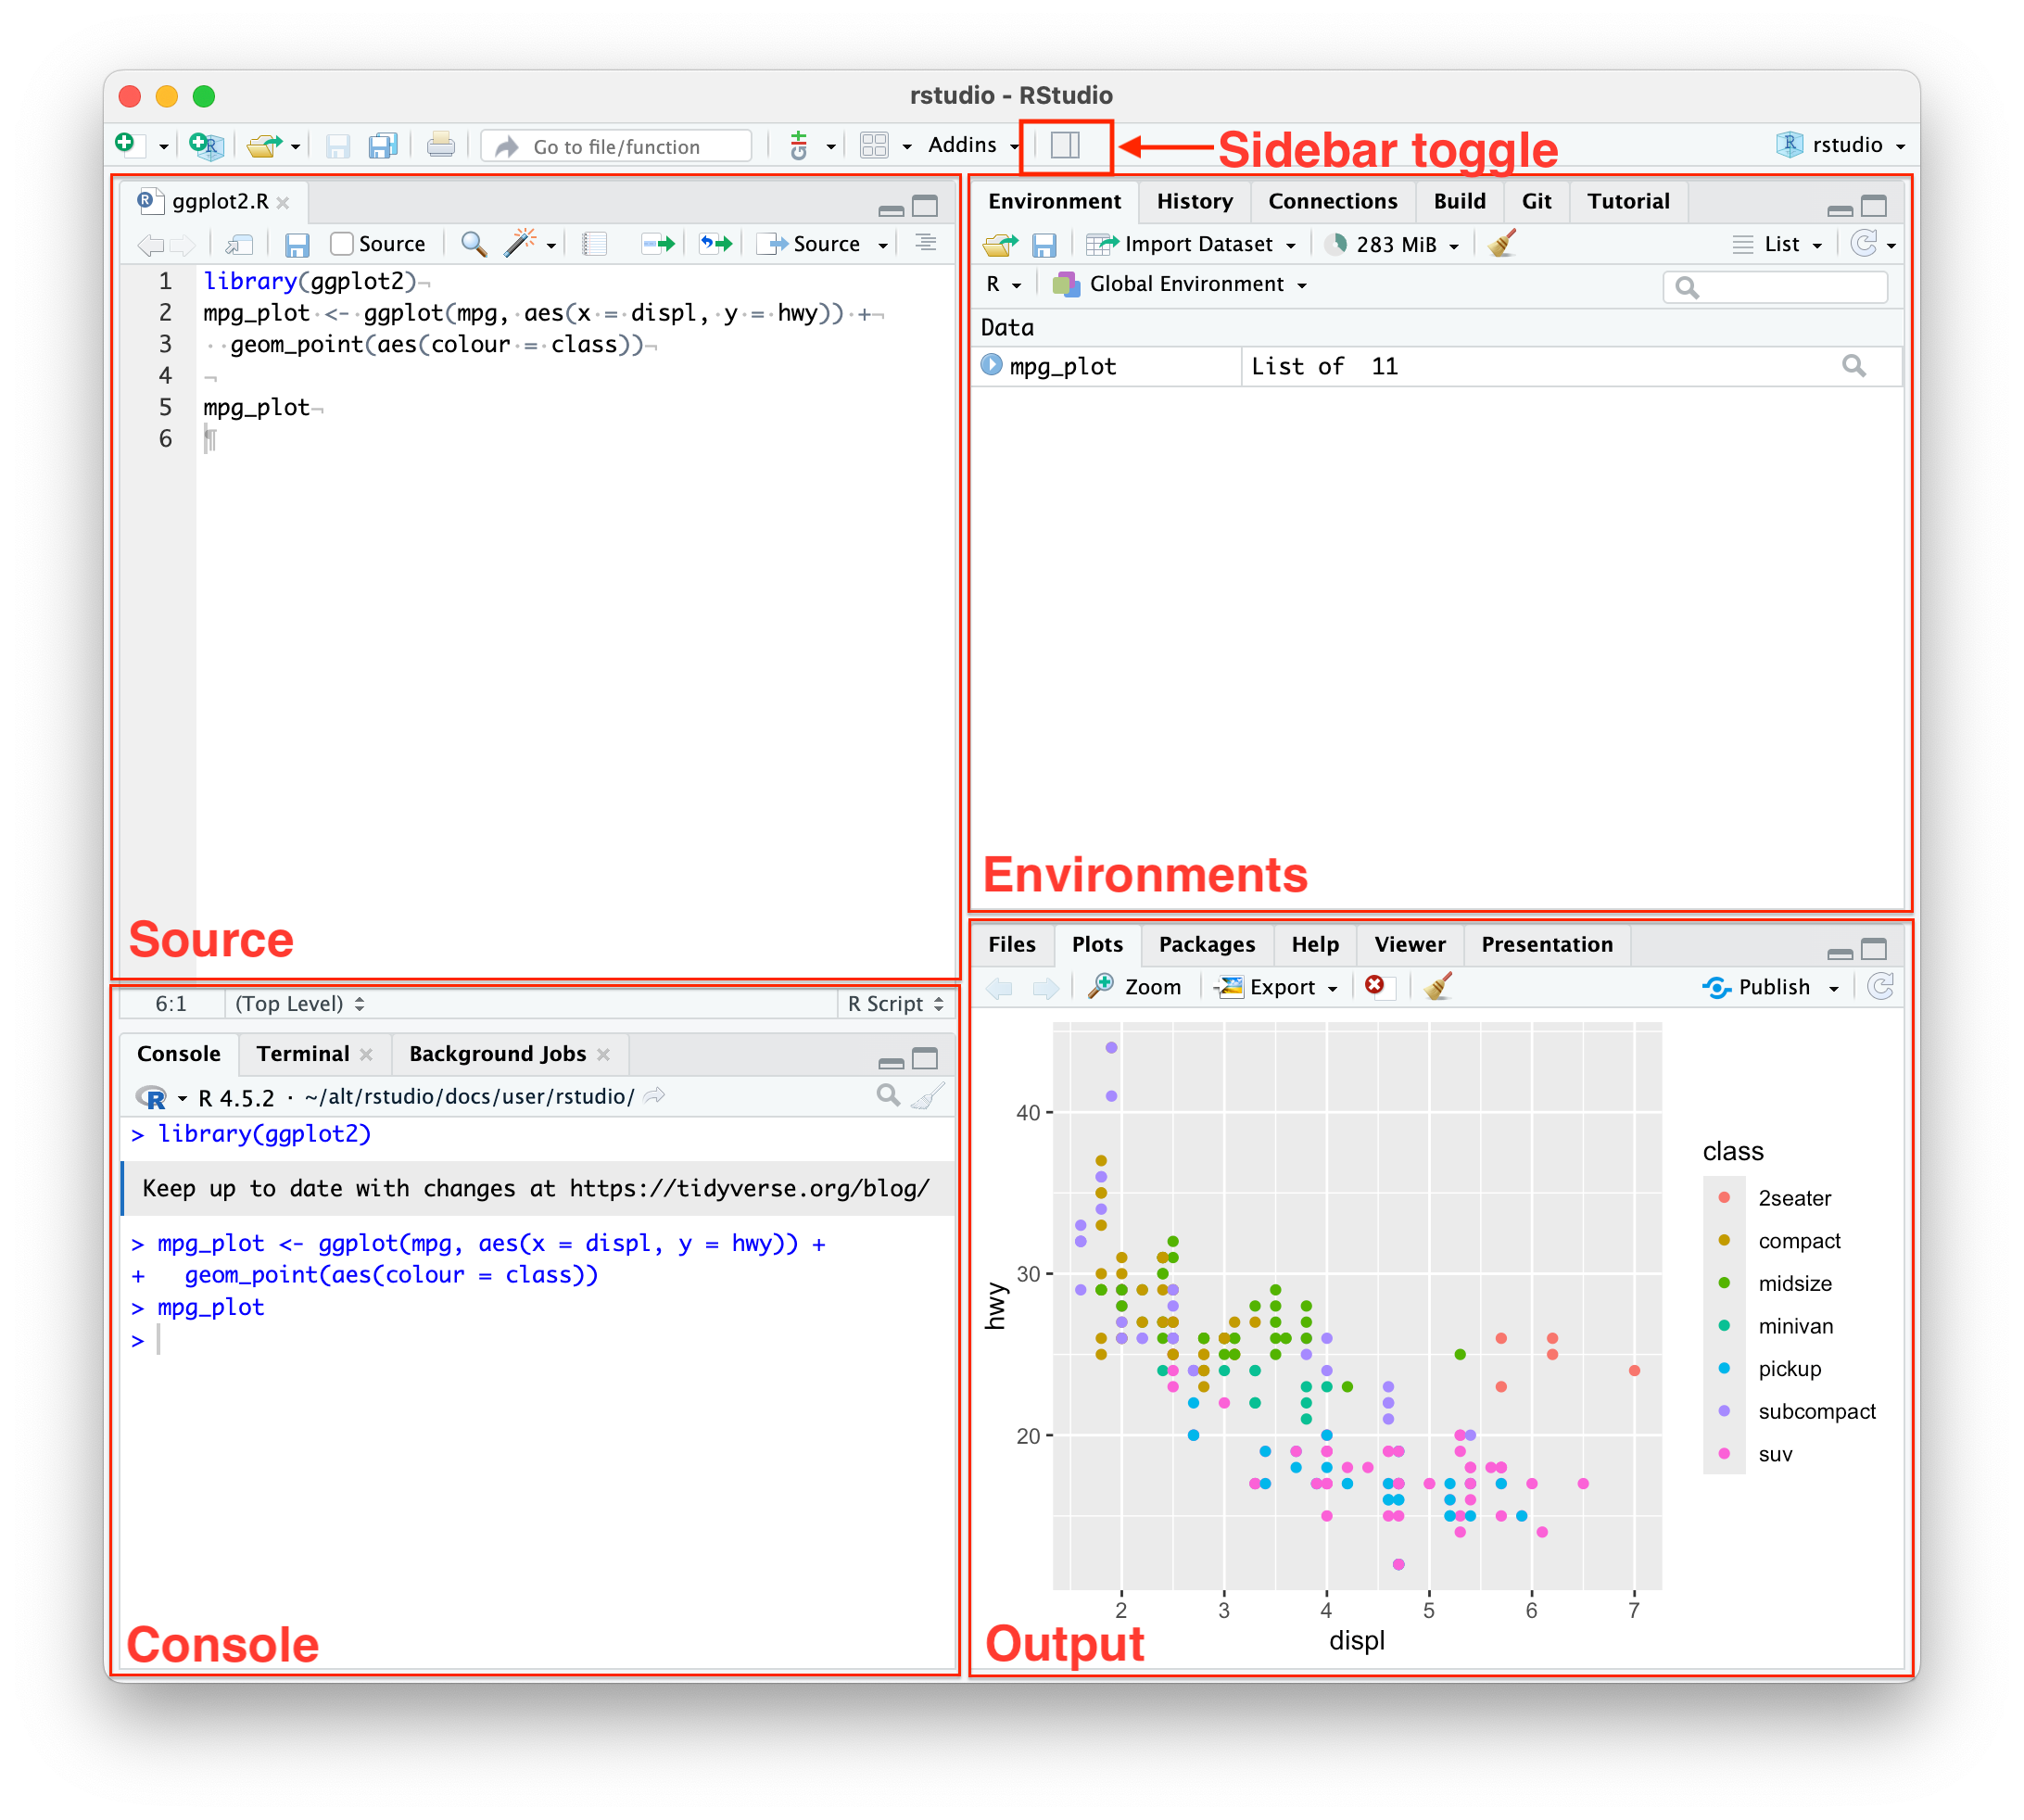
\includegraphics[width=0.65\linewidth,height=\textheight,keepaspectratio]{img/RStudio_layout.png}

Disposition des volets \textbf{RStudio}. \emph{Source :
\href{https://docs.posit.co/ide/user/ide/guide/ui/ui-panes.html}{RStudio
User Guide Release 2026.08.2} - Dernier accès : 2026-09-08}

\begin{center}\rule{0.5\linewidth}{0.5pt}\end{center}

\paragraph{1. Les scripts}\label{les-scripts}

Des fichiers ``texte'' pour des traitements qui vont nécessiter des
modifications.

\textbf{Avantages}

\begin{itemize}
\tightlist
\item
  garder la trace des lignes de code
\item
  exécuter une/des ligne(s) de code : bouton \texttt{Run} ou raccourci
  clavier \texttt{Ctrl\ +\ Entrée} ou \texttt{Ctrl\ +\ R}
\item
  modifier le code
\item
  ajouter des commentaires
\item
  réutiliser le code sur d'autres jeux de données
\end{itemize}

\begin{center}\rule{0.5\linewidth}{0.5pt}\end{center}

\paragraph{2. L'environnement / L'historique / Les
connexions}\label{lenvironnement-lhistorique-les-connexions}

\begin{itemize}
\item
  Onglet \textbf{Environment}

  \begin{itemize}
  \tightlist
  \item
    objets (données, fonctions, résultats) créés dans cet environnement
  \item
    2 affichages possibles : liste ou grille (permet de supprimer des
    objets en cochant la case à côté du nom + clic sur l'icone
    \texttt{Balai})
  \end{itemize}
\item
  Onglet \textbf{History}

  \begin{itemize}
  \tightlist
  \item
    historique des commandes exécutées
  \item
    on peut renvoyer le code dans la console ou la source
  \end{itemize}
\item
  Onglet \textbf{Connections}

  \begin{itemize}
  \tightlist
  \item
    pour se connecter à diverses sources de données (par ex. bases de
    données externes)
  \end{itemize}
\end{itemize}

\begin{center}\rule{0.5\linewidth}{0.5pt}\end{center}

\paragraph{3. La console}\label{la-console}

\textbf{C'est l'équivalent d'une calculatrice}

\begin{itemize}
\tightlist
\item
  Sert à effectuer et afficher les résultats de calculs de base
  (\texttt{+}, \texttt{-}, \texttt{\textbackslash{}*}, \texttt{/}, etc.
  )
\item
  Possibilité d'utiliser des fonctions spécifiques : \texttt{sum()},
  \texttt{abs()}, \texttt{round()}, etc.
\item
  Les commandes sont exécutées au fur et à mesure qu'elles sont écrites
  en appuyant sur la touche \texttt{Entrée}
\end{itemize}

\begin{tcolorbox}[enhanced jigsaw, arc=.35mm, bottomrule=.15mm, bottomtitle=1mm, breakable, colback=white, colbacktitle=quarto-callout-tip-color!10!white, colframe=quarto-callout-tip-color-frame, coltitle=black, left=2mm, leftrule=.75mm, opacityback=0, opacitybacktitle=0.6, rightrule=.15mm, title=\textcolor{quarto-callout-tip-color}{\faLightbulb}\hspace{0.5em}{Astuce}, titlerule=0mm, toprule=.15mm, toptitle=1mm]

\textbf{On peut naviguer dans l'historique des commandes pour en
rappeler une, à l'aide des flèches \(\uparrow\) et \(\downarrow\)}

\end{tcolorbox}

\begin{center}\rule{0.5\linewidth}{0.5pt}\end{center}

\paragraph{4. Les graphiques/ Les packages /
L'aide}\label{les-graphiques-les-packages-laide}

\begin{itemize}
\item
  Onglet \textbf{Plots}

  \begin{itemize}
  \tightlist
  \item
    fenêtre où s'affichent les graphiques que l'on crée dans les scripts
    (ou la console)
  \item
    possibilité de zoomer, de naviguer entre les graphiques, de les
    copier
  \item
    export des graphiques au format image (jpeg, png, tiff) ou pdf
  \end{itemize}
\item
  Onglet \textbf{Packages}

  \begin{itemize}
  \tightlist
  \item
    liste des packages installés sur la machine
  \item
    installation de nouveaux packages / mise à jour des packages
    installés
  \item
    un clic sur le nom d'un package affiche les pages d'aide de ce
    package
  \end{itemize}
\item
  Onglet \textbf{Help}

  \begin{itemize}
  \tightlist
  \item
    afficher la documentation de chaque fonction
  \item
    accéder à des manuels ou des à aides-mémoire (\emph{cheatsheets})
  \end{itemize}
\end{itemize}

\begin{center}\rule{0.5\linewidth}{0.5pt}\end{center}

\begin{tcolorbox}[enhanced jigsaw, arc=.35mm, bottomrule=.15mm, bottomtitle=1mm, breakable, colback=white, colbacktitle=quarto-callout-tip-color!10!white, colframe=quarto-callout-tip-color-frame, coltitle=black, left=2mm, leftrule=.75mm, opacityback=0, opacitybacktitle=0.6, rightrule=.15mm, title=\textcolor{quarto-callout-tip-color}{\faLightbulb}\hspace{0.5em}{Comment installer les logiciels ?}, titlerule=0mm, toprule=.15mm, toptitle=1mm]

L'installation se fait \textbf{dans cet ordre}

\begin{enumerate}
\def\labelenumi{\arabic{enumi}.}
\tightlist
\item
  \textbf{R} à partir du \href{http://cran.r-project.org}{CRAN}
  (\emph{Comprehensive R Archive Network})
\item
  \textbf{RStudio} via le site de
  \href{https://posit.co/downloads}{Posit}
\end{enumerate}

Le logiciel \textbf{R} est régulièrement mis à jour, et contrairement à
\textbf{RStudio}, il n'y a pas de message d'alerte pour vous prévenir.


\includegraphics[width=0.75em,height=1em]{index_files/figure-pdf/fa-icon-04c6f9870c69c7270c705a206c46d917.pdf}
\textbf{Pensez à vérifier régulièrement et à mettre à jour R pour
pouvoir bénéficier des dernières fonctionnalités !}

\end{tcolorbox}

\subsubsection{Les packages}\label{les-packages}

\begin{itemize}
\tightlist
\item
  Bibliothèques de fonctions et de données, développées par la
  communauté
\item
  Améliorent les fonctionnalités de base de \textbf{R} ou proposent des
  fonctionnalités supplémentaires
\item
  Contiennent de la documentation sur les fonctions qu'ils proposent
\end{itemize}

\emph{Exemple} : {\{ggplot2\}}, {\{dplyr\}}, {\{graphics\}}

\begin{center}\rule{0.5\linewidth}{0.5pt}\end{center}

\paragraph{\texorpdfstring{\textbf{Installer} un
package}{Installer un package}}\label{installer-un-package}

\textbf{L'installation d'un package dépend de l'endroit où les auteurs
l'ont déposé}

\begin{itemize}
\tightlist
\item
  Si le package est sur le CRAN, l'installation se fait avec la fonction
  \texttt{install.packages()}
\end{itemize}

\begin{Shaded}
\begin{Highlighting}[]
\CommentTok{\# Installer le package ggplot2}
\FunctionTok{install.packages}\NormalTok{(}\StringTok{"ggplot2"}\NormalTok{)}
\end{Highlighting}
\end{Shaded}

\begin{itemize}
\item
  Si les packages sont sur des dépôts, l'installation se fait grâce au
  package \href{https://remotes.r-lib.org/}{{\{remotes\}}}, avec des
  fonctions qui dépendent du dépôt

  \begin{itemize}
  \tightlist
  \item
    GitHub : fonction \texttt{install\_github()}
  \item
    GitLab : fonction \texttt{install\_gitlab()}
  \end{itemize}
\end{itemize}

\begin{Shaded}
\begin{Highlighting}[]
\CommentTok{\# Installer le package viewxl qui se trouve sur un dépôt Github}
\NormalTok{remotes}\SpecialCharTok{::}\FunctionTok{install\_github}\NormalTok{(}\StringTok{"dreamRs/viewxl"}\NormalTok{)}
\end{Highlighting}
\end{Shaded}

\begin{tcolorbox}[enhanced jigsaw, arc=.35mm, bottomrule=.15mm, breakable, colback=white, colframe=quarto-callout-tip-color-frame, left=2mm, leftrule=.75mm, opacityback=0, rightrule=.15mm, toprule=.15mm]
\begin{minipage}[t]{5.5mm}
\textcolor{quarto-callout-tip-color}{\faLightbulb}
\end{minipage}%
\begin{minipage}[t]{\textwidth - 5.5mm}

\textbf{L'installation ne doit pas être refaite à chaque exécution du
script !}

\end{minipage}%
\end{tcolorbox}

\begin{center}\rule{0.5\linewidth}{0.5pt}\end{center}

\paragraph{\texorpdfstring{\textbf{Charger} un
package}{Charger un package}}\label{charger-un-package}

\textbf{Cette étape est nécessaire à chaque fois que l'on veut utiliser
une ou plusieurs fonctions d'un package}

\begin{Shaded}
\begin{Highlighting}[]
\CommentTok{\# Charger le package ggplot2}
\FunctionTok{library}\NormalTok{(ggplot2)}
\end{Highlighting}
\end{Shaded}

\begin{tcolorbox}[enhanced jigsaw, arc=.35mm, bottomrule=.15mm, bottomtitle=1mm, breakable, colback=white, colbacktitle=quarto-callout-warning-color!10!white, colframe=quarto-callout-warning-color-frame, coltitle=black, left=2mm, leftrule=.75mm, opacityback=0, opacitybacktitle=0.6, rightrule=.15mm, title=\textcolor{quarto-callout-warning-color}{\faExclamationTriangle}\hspace{0.5em}{La gestion des packages}, titlerule=0mm, toprule=.15mm, toptitle=1mm]

Les packages évoluent, les fonctions changent et avec une nouvelle
version de package, votre code peut ne plus s'exécuter sans erreur


\includegraphics[width=0.75em,height=1em]{index_files/figure-pdf/fa-icon-04c6f9870c69c7270c705a206c46d917.pdf}
\textbf{Il est vivement recommandé de lister les packages utilisés au
début de vos scripts, pour les identifier plus rapidement, en notant
leur version}

\begin{itemize}
\tightlist
\item
  ``à la main''
\end{itemize}

\begin{Shaded}
\begin{Highlighting}[]
\FunctionTok{library}\NormalTok{(tidyverse)    }\CommentTok{\# v2.0.0}
\FunctionTok{library}\NormalTok{(questionr)    }\CommentTok{\# v0.8.2}
\end{Highlighting}
\end{Shaded}

\begin{itemize}
\tightlist
\item
  de façon automatique
\end{itemize}

\begin{Shaded}
\begin{Highlighting}[]
\FunctionTok{library}\NormalTok{(tidyverse)}
\FunctionTok{library}\NormalTok{(questionr)}

\NormalTok{packages\_utilises }\OtherTok{\textless{}{-}} \FunctionTok{sessionInfo}\NormalTok{()}
\end{Highlighting}
\end{Shaded}

\end{tcolorbox}

\begin{center}\rule{0.5\linewidth}{0.5pt}\end{center}

\paragraph{\texorpdfstring{Que se passe-t'il quand on installe une
nouvelle version de \textbf{R}
?}{Que se passe-t'il quand on installe une nouvelle version de R ?}}\label{que-se-passe-til-quand-on-installe-une-nouvelle-version-de-r}

\begin{itemize}
\tightlist
\item
  Seul les packages de base sont installés, dans leur version mise à
  jour
\item
  Les packages qui ont été installés en fonction des besoins ne le sont
  pas, il faut les réinstaller
\end{itemize}

\begin{tcolorbox}[enhanced jigsaw, arc=.35mm, bottomrule=.15mm, breakable, colback=white, colframe=quarto-callout-note-color-frame, left=2mm, leftrule=.75mm, opacityback=0, rightrule=.15mm, toprule=.15mm]
\begin{minipage}[t]{5.5mm}
\textcolor{quarto-callout-note-color}{\faInfo}
\end{minipage}%
\begin{minipage}[t]{\textwidth - 5.5mm}

\textbf{RStudio} affiche un avertissement en haut des scripts qui
appellent des packages qui ne sont pas installés

\end{minipage}%
\end{tcolorbox}

\subparagraph{Comment réinstaller les packages automatiquement
?}\label{comment-ruxe9installer-les-packages-automatiquement}

\textbf{Les étapes à suivre}

\begin{itemize}
\item
  Créer un script \textbf{R} qui va contenir la liste des packages à
  installer, quel que soit le projet dans lequel vous travaillez

  \begin{itemize}
  \tightlist
  \item
    pour les packages qui se trouvent sur le CRAN, lister les packages
    dans la commande \texttt{install.packages()}\\
  \item
    pour les packages qui se trouvent sur les dépôts GitHub,
    l'installation se fera avec la commande \texttt{install\_github()}
    du package \href{https://remotes.r-lib.org/}{{\{remotes\}}}
  \end{itemize}
\item
  Mettre à jour le script au fur et à mesure des installations de
  nouveaux packages
\item
  Exécuter le contenu du script, en ayant pris soin auparavant
  d'actualiser la version de \textbf{R} sous \textbf{RStudio} si
  plusieurs sont installées !
\end{itemize}

\begin{center}\rule{0.5\linewidth}{0.5pt}\end{center}

\emph{Exemple de script}

\begin{Shaded}
\begin{Highlighting}[]
\CommentTok{\#   \_\_\_\_\_\_\_\_\_\_\_\_\_\_\_\_\_\_\_\_\_\_\_\_\_\_\_\_\_\_\_\_\_\_\_\_\_\_\_\_\_\_\_\_\_\_\_\_\_\_\_\_\_\_\_\_\_\_\_\_\_\_\_\_\_\_\_\_\_\_\_\_\_\_\_\_}
\CommentTok{\#   Script: Packages à installer après chaque nouvelle installation de R}
\CommentTok{\#   Author: Sandrine.Lyser}
\CommentTok{\#   Créé le : 2026{-}06{-}19}
\CommentTok{\#   Dernière modification : 2026{-}09{-}07}
\CommentTok{\#   Text defaut encoding : UTF{-}8}
\CommentTok{\#   \_\_\_\_\_\_\_\_\_\_\_\_\_\_\_\_\_\_\_\_\_\_\_\_\_\_\_\_\_\_\_\_\_\_\_\_\_\_\_\_\_\_\_\_\_\_\_\_\_\_\_\_\_\_\_\_\_\_\_\_\_\_\_\_\_\_\_\_\_\_\_\_\_\_\_\_}


\CommentTok{\# Packages du CRAN}
\FunctionTok{install.packages}\NormalTok{(}\FunctionTok{c}\NormalTok{(}\StringTok{"tidyverse"}\NormalTok{, }\StringTok{"esquisse"}\NormalTok{, }\StringTok{"RColorBrewer"}\NormalTok{, }\StringTok{"remotes"}\NormalTok{, }\StringTok{"mapsf"}\NormalTok{),}
                 \AttributeTok{dependencies =} \ConstantTok{TRUE}\NormalTok{)}

\CommentTok{\# Autres packages (sur github par exemple)}
\NormalTok{remotes}\SpecialCharTok{::}\FunctionTok{install\_github}\NormalTok{(}\StringTok{"lorenzwalthert/strcode"}\NormalTok{, }\AttributeTok{dependencies =} \ConstantTok{TRUE}\NormalTok{)}
                        
\NormalTok{remotes}\SpecialCharTok{::}\FunctionTok{install\_github}\NormalTok{(}\StringTok{"dreamRs/viewxl"}\NormalTok{, }\AttributeTok{dependencies =} \ConstantTok{TRUE}\NormalTok{)}
\end{Highlighting}
\end{Shaded}

\begin{center}\rule{0.5\linewidth}{0.5pt}\end{center}

\begin{tcolorbox}[enhanced jigsaw, arc=.35mm, bottomrule=.15mm, bottomtitle=1mm, breakable, colback=white, colbacktitle=quarto-callout-note-color!10!white, colframe=quarto-callout-note-color-frame, coltitle=black, left=2mm, leftrule=.75mm, opacityback=0, opacitybacktitle=0.6, rightrule=.15mm, title=\textcolor{quarto-callout-note-color}{\faInfo}\hspace{0.5em}{Le préfixage}, titlerule=0mm, toprule=.15mm, toptitle=1mm]

La notation

\begin{Shaded}
\begin{Highlighting}[]
\NormalTok{dplyr}\SpecialCharTok{::}\FunctionTok{filter}\NormalTok{(Journals, field }\SpecialCharTok{==} \StringTok{"Econometrics"}\NormalTok{)}
\end{Highlighting}
\end{Shaded}

peut remplacer le code

\begin{Shaded}
\begin{Highlighting}[]
\FunctionTok{library}\NormalTok{(dplyr)}
\FunctionTok{filter}\NormalTok{(Journals, field }\SpecialCharTok{==} \StringTok{"Econometrics"}\NormalTok{)}
\end{Highlighting}
\end{Shaded}

\textbf{Avantages}

\begin{itemize}
\tightlist
\item
  Évite les conflits si plusieurs packages ont une fonction avec le même
  nom (mais des paramètres différents)\\
  \emph{Exemple} la fonction \texttt{filter()} existe dans les packages
  \{stats\} et \{dplyr\}
\item
  Identifie le package d'où provient une fonction
\item
  Ne charge pas la totalité d'un package pour n'utiliser qu'une seule de
  ses fonctions
\end{itemize}

\end{tcolorbox}

\begin{center}\rule{0.5\linewidth}{0.5pt}\end{center}

\begin{tcolorbox}[enhanced jigsaw, arc=.35mm, bottomrule=.15mm, bottomtitle=1mm, breakable, colback=white, colbacktitle=quarto-callout-tip-color!10!white, colframe=quarto-callout-tip-color-frame, coltitle=black, left=2mm, leftrule=.75mm, opacityback=0, opacitybacktitle=0.6, rightrule=.15mm, title=\textcolor{quarto-callout-tip-color}{\faLightbulb}\hspace{0.5em}{Vous ne savez pas comment faire pour citer \textbf{R} ainsi que les
packages que vous avez utilisés dans vos travaux ?}, titlerule=0mm, toprule=.15mm, toptitle=1mm]

La fonction \texttt{citation()} est là pour vous aider !

\begin{itemize}
\tightlist
\item
  \textbf{Pour citer la version de R}
\end{itemize}

\begin{Shaded}
\begin{Highlighting}[]
\CommentTok{\# Citer R}
\FunctionTok{citation}\NormalTok{()}
\end{Highlighting}
\end{Shaded}

\begin{verbatim}
To cite R in publications use:

  R Core Team (2026). _R: A Language and Environment for Statistical
  Computing_. R Foundation for Statistical Computing, Vienna, Austria.
  doi:10.32614/R.manuals <https://doi.org/10.32614/R.manuals>.
  <https://www.R-project.org/>.

Une entrée BibTeX pour les utilisateurs LaTeX est

  @Manual{,
    title = {R: A Language and Environment for Statistical Computing},
    author = {{R Core Team}},
    organization = {R Foundation for Statistical Computing},
    address = {Vienna, Austria},
    year = {2026},
    doi = {10.32614/R.manuals},
    url = {https://www.R-project.org/},
  }

We have invested a lot of time and effort in creating R, please cite it
when using it for data analysis. See also 'citation("pkgname")' for
citing R packages.
\end{verbatim}

\begin{itemize}
\tightlist
\item
  \textbf{Pour citer un package}
\end{itemize}

\begin{Shaded}
\begin{Highlighting}[]
\CommentTok{\# Citer un package (ici ggplot2)}
\FunctionTok{citation}\NormalTok{(}\StringTok{"ggplot2"}\NormalTok{)}
\end{Highlighting}
\end{Shaded}

\begin{verbatim}
To cite ggplot2 in publications, please use

  H. Wickham. ggplot2: Elegant Graphics for Data Analysis.
  Springer-Verlag New York, 2016.

Une entrée BibTeX pour les utilisateurs LaTeX est

  @Book{,
    author = {Hadley Wickham},
    title = {ggplot2: Elegant Graphics for Data Analysis},
    publisher = {Springer-Verlag New York},
    year = {2016},
    isbn = {978-3-319-24277-4},
    url = {https://ggplot2.tidyverse.org},
  }
\end{verbatim}

\end{tcolorbox}

\section{\texorpdfstring{Travailler avec les projets \textbf{RStudio} et
reproductibilité}{Travailler avec les projets RStudio et reproductibilité}}\label{travailler-avec-les-projets-rstudio-et-reproductibilituxe9}

\subsection{Qu'est-ce que la reproductibilité en science des données
?}\label{quest-ce-que-la-reproductibilituxe9-en-science-des-donnuxe9es}

\textbf{= Processus qui peut être reproduit par une autre personne et/ou
à partir des mêmes données mises à jour et qui permet d'expliquer et
partager son travail}

S'appuie sur \textbf{trois grands principes} interagissant entre eux et
non séquentiels\footnote{Orozco, V., C. Bontemps, E. Maigné, V. Piguet,
  A. Hofstetter, A. Lacroix, F. Levert, and J-M. Rousselle. 2020. ``How
  To Make A Pie: Reproducible Research for Empirical Economics and
  Econometrics.'' Journal of Economic Surveys 34 (5) : 1134--69.
  https://doi.org/10.1111/joes.12389.}

\begin{enumerate}
\def\labelenumi{\arabic{enumi}.}
\tightlist
\item
  Organiser son travail
\item
  Coder pour les autres
\item
  Automatiser le plus possible
\end{enumerate}

\begin{center}\rule{0.5\linewidth}{0.5pt}\end{center}

\subsubsection{\texorpdfstring{Comment travailler de façon reproductible
sous \textbf{R} et \textbf{RStudio}
?}{Comment travailler de façon reproductible sous R et RStudio ?}}\label{comment-travailler-de-fauxe7on-reproductible-sous-r-et-rstudio}

\begin{enumerate}
\def\labelenumi{\arabic{enumi}.}
\tightlist
\item
  En utilisant les \textbf{projets RStudio} : on isole chaque analyse
\item
  En stockant ses traitements dans des \textbf{scripts R} : on garde une
  trace des commandes, pas de travail dans la console
\item
  En utilisant les \textbf{chemins relatifs} : pour exécuter sans
  problème le code sur un autre ordinateur
\item
  En prêtant une attention à la \textbf{gestion des packages} : versions
  et dépendances
\item
  En \textbf{documentant} son travail : commentaires, fichier README
\end{enumerate}

\begin{center}\rule{0.5\linewidth}{0.5pt}\end{center}

\begin{tcolorbox}[enhanced jigsaw, arc=.35mm, bottomrule=.15mm, bottomtitle=1mm, breakable, colback=white, colbacktitle=quarto-callout-note-color!10!white, colframe=quarto-callout-note-color-frame, coltitle=black, left=2mm, leftrule=.75mm, opacityback=0, opacitybacktitle=0.6, rightrule=.15mm, title=\textcolor{quarto-callout-note-color}{\faInfo}\hspace{0.5em}{Zoom sur l'encodage}, titlerule=0mm, toprule=.15mm, toptitle=1mm]

\textbf{L'encodage est un processus de conversion d'informations (texte,
données, etc.) en un format lisible, compréhensible et exploitable par
différents systèmes} \(\Rightarrow\) il permet une compatibilité entre
systèmes

\begin{itemize}
\tightlist
\item
  Il existe plusieurs encodages, comme par exemple : ASCII, ISO 8859-15,
  UTF-8
\item
  Les encodages sont différents selon le système d'exploitation
  (Windows-1252 sous Windows, UTF-8 sous Linux ou Mac)
\end{itemize}


\includegraphics[width=0.75em,height=1em]{index_files/figure-pdf/fa-icon-04c6f9870c69c7270c705a206c46d917.pdf}
\textbf{Il est recommandé d'utiliser l'encodage UTF-8 pour les scripts
et les données}, car c'est à l'heure actuelle l'encodage le plus
universel


\includegraphics[width=1.25em,height=1em]{index_files/figure-pdf/fa-icon-6e3e6b566131db41246b1ca486a392da.pdf}
\textbf{Comment peut-on définir l'encodage sous RStudio ?}\\
- Allez dans
\texttt{Tools\ \textgreater{}\ Global\ Options\ \textgreater{}\ Code\ \textgreater{}\ Saving\ \textgreater{}\ Default\ text\ encoding}\\
- Sélectionnez \texttt{UTF-8}

\end{tcolorbox}

\begin{center}\rule{0.5\linewidth}{0.5pt}\end{center}

\begin{tcolorbox}[enhanced jigsaw, arc=.35mm, bottomrule=.15mm, bottomtitle=1mm, breakable, colback=white, colbacktitle=quarto-callout-tip-color!10!white, colframe=quarto-callout-tip-color-frame, coltitle=black, left=2mm, leftrule=.75mm, opacityback=0, opacitybacktitle=0.6, rightrule=.15mm, title=\textcolor{quarto-callout-tip-color}{\faLightbulb}\hspace{0.5em}{La fonction \texttt{set.seed()}}, titlerule=0mm, toprule=.15mm, toptitle=1mm]

\textbf{Automatiser c'est aussi pouvoir refaire les mêmes calculs et
obtenir les mêmes résultats}

\(\Rightarrow\) utiliser la fonction \texttt{set.seed()} permet de
garantir la reproductibilité des résultats de tout travail inscrit dans
un script \textbf{R} qui implique de l'aléatoire (simulation
permutation, bootstrap, etc.)


\includegraphics[width=0.75em,height=1em]{index_files/figure-pdf/fa-icon-04c6f9870c69c7270c705a206c46d917.pdf}
\textbf{Placée avant une opération aléatoire (fonctions
\texttt{sample()}, \texttt{rnorm()} par exemple), elle permet de
retrouver les mêmes résultats à chaque exécution}

\begin{Shaded}
\begin{Highlighting}[]
\FunctionTok{set.seed}\NormalTok{(}\DecValTok{123}\NormalTok{)     }\CommentTok{\# \textquotesingle{}Graine\textquotesingle{} (valeur quelconque) pour le générateur aléatoire}
\FunctionTok{sample}\NormalTok{(}\DecValTok{1}\SpecialCharTok{:}\DecValTok{10}\NormalTok{, }\DecValTok{5}\NormalTok{)   }\CommentTok{\# Un tirage reproductible}
\end{Highlighting}
\end{Shaded}

\begin{verbatim}
[1]  3 10  2  8  6
\end{verbatim}

\end{tcolorbox}

\subsubsection{\texorpdfstring{Les projets
\textbf{RStudio}}{Les projets RStudio}}\label{les-projets-rstudio}

Les projets \textbf{RStudio} sont utiles pour

\begin{itemize}
\tightlist
\item
  \textbf{organiser plus facilement son travail} : 1 projet
  \textbf{RStudio} = 1 projet de recherche / 1 étude / 1 cours, etc.\\
  \(\Rightarrow\) environnement isolé, pas de conflits entre projets
\item
  \textbf{regrouper dans un même dossier tous les scripts} : scripts
  \textbf{R}/quarto, fonctions, données, résultats, graphiques, etc.
\item
  \textbf{améliorer la portabilité et faciliter les collaborations} :
  utilisation des chemins de fichiers relatifs \(\Rightarrow\)
  reproductibilité facilitée
\end{itemize}

\begin{tcolorbox}[enhanced jigsaw, arc=.35mm, bottomrule=.15mm, bottomtitle=1mm, breakable, colback=white, colbacktitle=quarto-callout-note-color!10!white, colframe=quarto-callout-note-color-frame, coltitle=black, left=2mm, leftrule=.75mm, opacityback=0, opacitybacktitle=0.6, rightrule=.15mm, title=\textcolor{quarto-callout-note-color}{\faInfo}\hspace{0.5em}{Chemins absolus/relatifs}, titlerule=0mm, toprule=.15mm, toptitle=1mm]

\begin{itemize}
\item
  Le chemin absolu est exprimé par rapport au disque dur, à
  l'ordinateur\\
  \emph{Exemple} : \texttt{C:/Users/...}
\item
  Le chemin relatif est exprimé par rapport au projet\\
  \emph{Exemple} : \texttt{data/mon\_fichier.csv}
\end{itemize}


\includegraphics[width=0.75em,height=1em]{index_files/figure-pdf/fa-icon-04c6f9870c69c7270c705a206c46d917.pdf}
\textbf{Le répertoire par défaut du projet est le dossier où est
enregistré le projet sur votre machine}

\end{tcolorbox}

\begin{center}\rule{0.5\linewidth}{0.5pt}\end{center}

\paragraph{Comment créer un projet ?}\label{comment-cruxe9er-un-projet}

À partir de l'icône dédiée en haut à droite de \textbf{RStudio}

\begin{center}
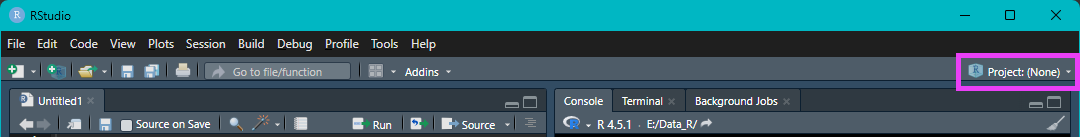
\includegraphics[width=0.65\linewidth,height=\textheight,keepaspectratio]{img/screenshot_RStudio_NewProject.png}
\end{center}

Cliquez sur
\texttt{New\ Project\ \textgreater{}\ New\ Directory\ \textgreater{}\ New\ Project}
et complétez les informations requises

\begin{itemize}
\tightlist
\item
  le nom du dossier/projet
\item
  son emplacement (dossier de votre choix)
\end{itemize}

\begin{center}
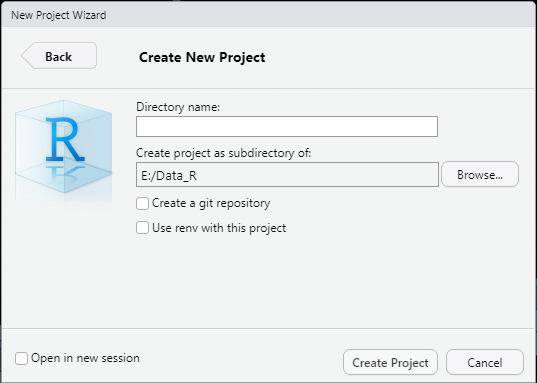
\includegraphics[width=0.55\linewidth,height=\textheight,keepaspectratio]{img/screenshot_RStudio_ProjectDirectory.png}
\end{center}

\begin{tcolorbox}[enhanced jigsaw, arc=.35mm, bottomrule=.15mm, breakable, colback=white, colframe=quarto-callout-tip-color-frame, left=2mm, leftrule=.75mm, opacityback=0, rightrule=.15mm, toprule=.15mm]
\begin{minipage}[t]{5.5mm}
\textcolor{quarto-callout-tip-color}{\faLightbulb}
\end{minipage}%
\begin{minipage}[t]{\textwidth - 5.5mm}

\textbf{Quand le projet est créé}\\
- \textbf{RStudio} redémarre et se place dans ce projet\\
- le projet apparaît dans l'onglet \emph{Files} de \textbf{RStudio}


\includegraphics[width=0.75em,height=1em]{index_files/figure-pdf/fa-icon-04c6f9870c69c7270c705a206c46d917.pdf}
Pour ranger efficacement les différents documents liés à l'analyse, vous
pouvez créer les sous-dossiers\\
- soit en cliquant sur \texttt{New\ Folder} dans le menu en haut de
l'onglet \emph{Files}\\
- soit de façon classique, à partir de l'explorateur de fichier de votre
machine

\end{minipage}%
\end{tcolorbox}

\begin{center}\rule{0.5\linewidth}{0.5pt}\end{center}

\paragraph{Comment structurer ses projets
?}\label{comment-structurer-ses-projets}

\textbf{Choisissez la structuration qui vous correspond le mieux} pour
\textbf{rassembler} tous les éléments liés au projet dans des
dossiers/sous-dossiers qui séparent données source/créées, scripts,
documentation, résultats, etc.

\begin{tcolorbox}[enhanced jigsaw, arc=.35mm, bottomrule=.15mm, breakable, colback=white, colframe=quarto-callout-tip-color-frame, left=2mm, leftrule=.75mm, opacityback=0, rightrule=.15mm, toprule=.15mm]
\begin{minipage}[t]{5.5mm}
\textcolor{quarto-callout-tip-color}{\faLightbulb}
\end{minipage}%
\begin{minipage}[t]{\textwidth - 5.5mm}

\textbf{Chacun s'organise de la façon qu'il juge la plus adaptée à ses
usages, en gardant en tête que ce sont les données initiales et les
scripts de traitement qui sont les plus importants pour pouvoir rejouer
les analyses}

\end{minipage}%
\end{tcolorbox}

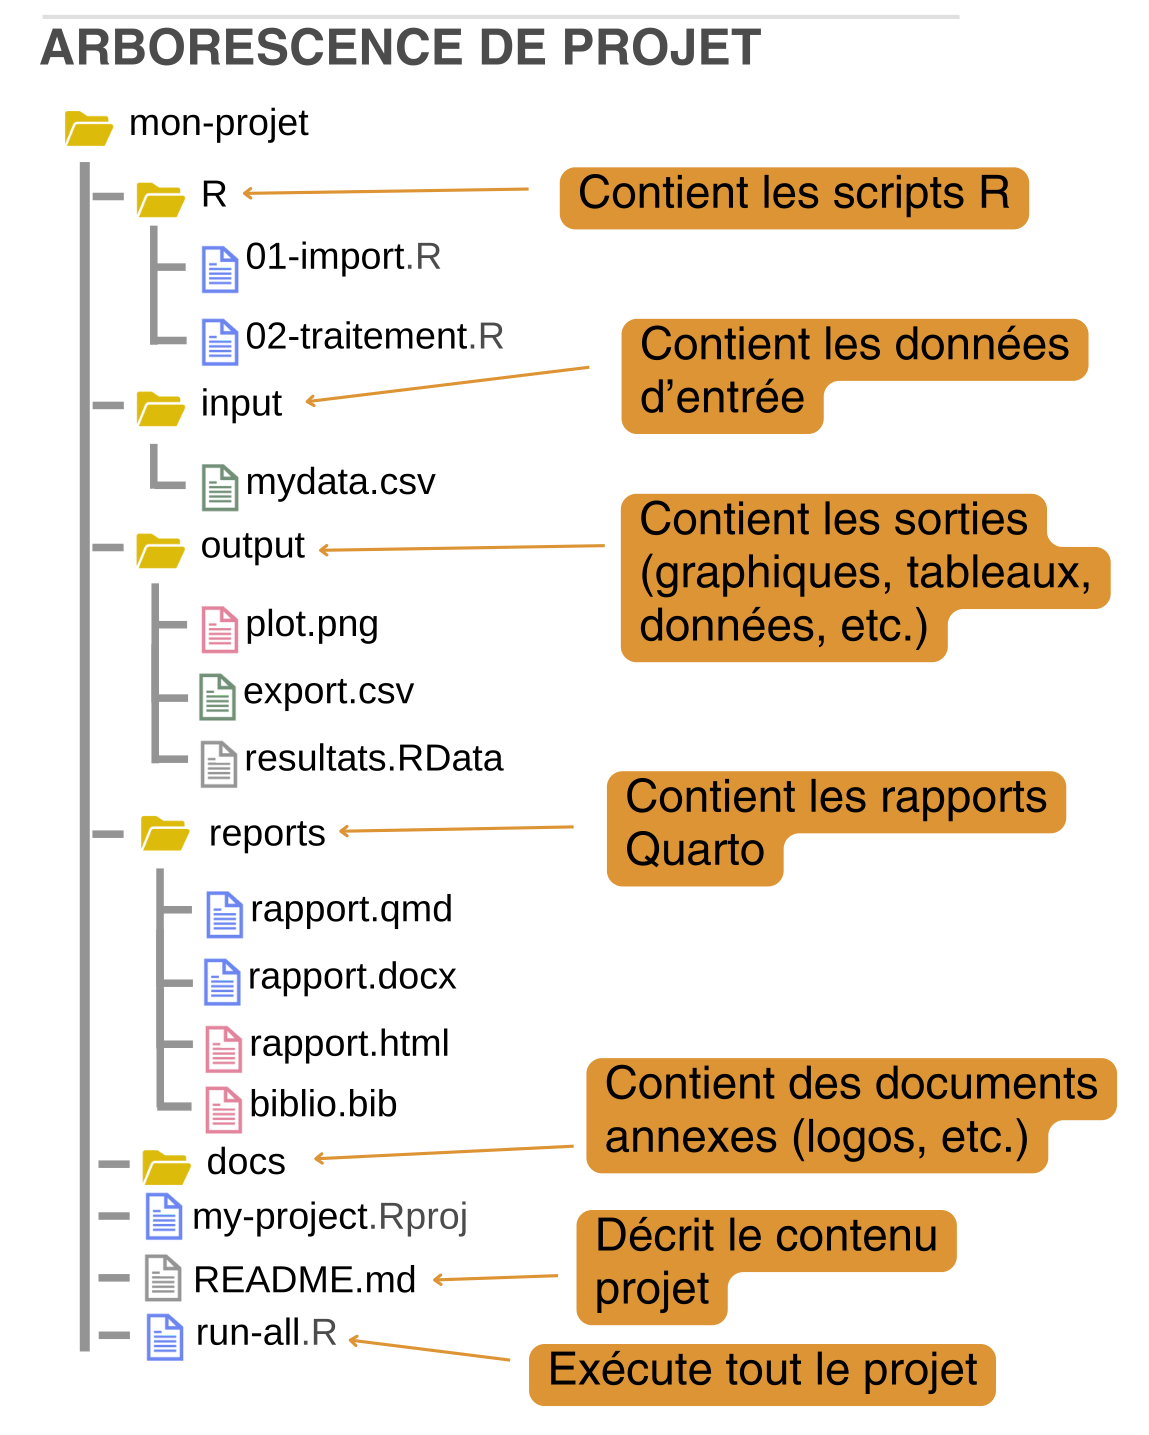
\includegraphics[width=0.33\linewidth,height=\textheight,keepaspectratio]{img/ProjectStructure.png}
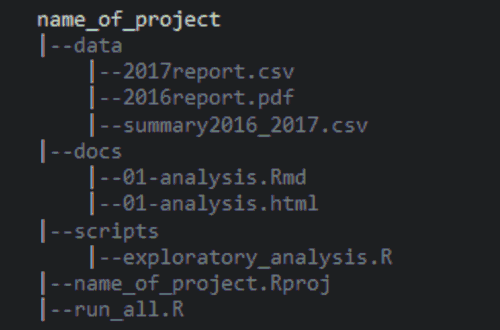
\includegraphics[width=0.33\linewidth,height=\textheight,keepaspectratio]{img/screenshot_RStudio_ProjectStructureMini.png}
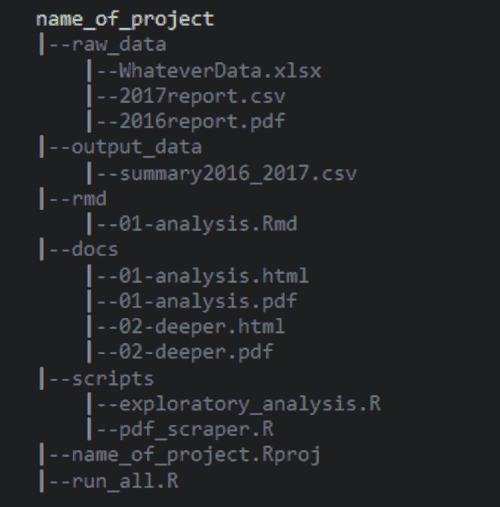
\includegraphics[width=0.33\linewidth,height=\textheight,keepaspectratio]{img/screenshot_RStudio_ProjectStructureOptim.png}

Exemples de structuration de projets \textbf{R} \emph{Source (figures 2
\& 3) :
\url{https://learn.r-journalism.com/en/publishing/workflow/r-projects/}
- Dernier accès : 2026-09-08}

\subsubsection{\texorpdfstring{Les scripts
\textbf{R}}{Les scripts R}}\label{les-scripts-r}

\begin{itemize}
\tightlist
\item
  Ils permettent de \textbf{garder la trace} du processus de création de
  chaque variable, tableau, figure, etc., ce qui permet de refaire les
  traitements dans leur globalité\\
\item
  Ils sont \textbf{facilement partageables} avec d'autres, sous réserve
  de respecter des pratiques de ``bon'' usage

  \begin{itemize}
  \tightlist
  \item
    coder de façon compréhensible avec des commentaires et en
    documentant ses fonctions\\
  \item
    donner des noms explicites aux objets et fonctions
  \item
    utiliser les conventions de nommage, notamment pour distinguer les
    variables d'origine des variables créées
  \end{itemize}
\end{itemize}

\begin{tcolorbox}[enhanced jigsaw, arc=.35mm, bottomrule=.15mm, breakable, colback=white, colframe=quarto-callout-tip-color-frame, left=2mm, leftrule=.75mm, opacityback=0, rightrule=.15mm, toprule=.15mm]
\begin{minipage}[t]{5.5mm}
\textcolor{quarto-callout-tip-color}{\faLightbulb}
\end{minipage}%
\begin{minipage}[t]{\textwidth - 5.5mm}

\begin{itemize}
\tightlist
\item
  Pour les \textbf{variables}, utiliser un \textbf{nom}\\
  \emph{Exemple} : \texttt{temperature\_max}
\item
  Pour les \textbf{fonctions}, utiliser un \textbf{verbe}\\
  \emph{Exemple} : \texttt{create.map} serait une fonction qui
  permettrait de créer une carte
\item
  Pour \textbf{distinguer variables d'origine / variables recodées}, on
  peut utiliser un préfixe ou un suffixe\\
  \emph{Exemple} : \texttt{age} est la variable d'origine et
  \texttt{age\_recod} est la variable recodée
\end{itemize}

\end{minipage}%
\end{tcolorbox}

\begin{center}\rule{0.5\linewidth}{0.5pt}\end{center}

\begin{tcolorbox}[enhanced jigsaw, arc=.35mm, bottomrule=.15mm, bottomtitle=1mm, breakable, colback=white, colbacktitle=quarto-callout-note-color!10!white, colframe=quarto-callout-note-color-frame, coltitle=black, left=2mm, leftrule=.75mm, opacityback=0, opacitybacktitle=0.6, rightrule=.15mm, title=\textcolor{quarto-callout-note-color}{\faInfo}\hspace{0.5em}{Les conventions de nommage}, titlerule=0mm, toprule=.15mm, toptitle=1mm]

Il existe différentes conventions

\begin{itemize}
\tightlist
\item
  \textbf{\texttt{allowercase}} : tout en minuscule, sans séparateur
\item
  \textbf{\texttt{period.separated}} : tout en minuscule, mots séparés
  par des points
\item
  \textbf{\texttt{underscore\_separated}} : tout en minuscule, mots
  séparés par un \emph{underscore} (\texttt{\_})
\item
  \textbf{\texttt{lowerCamelCase}} : première lettre des mots en
  majuscule, à l'exception du premier mot ; et si nom simple, tout en
  minuscule
\item
  \textbf{\texttt{UpperCamelCase}} : première lettre des mots en
  majuscule, y compris le premier et même lorsque le nom est composé
  d'un seul mot
\end{itemize}


\includegraphics[width=0.75em,height=1em]{index_files/figure-pdf/fa-icon-04c6f9870c69c7270c705a206c46d917.pdf}
\textbf{Possibilité de mixer les conventions mais en gardant une
cohérence afin de faciliter la compréhension des fichiers et du code}

\end{tcolorbox}

\begin{tcolorbox}[enhanced jigsaw, arc=.35mm, bottomrule=.15mm, breakable, colback=white, colframe=quarto-callout-warning-color-frame, left=2mm, leftrule=.75mm, opacityback=0, rightrule=.15mm, toprule=.15mm]
\begin{minipage}[t]{5.5mm}
\textcolor{quarto-callout-warning-color}{\faExclamationTriangle}
\end{minipage}%
\begin{minipage}[t]{\textwidth - 5.5mm}

\textbf{R est sensible à la casse} ce qui signifie que \texttt{variable}
et \texttt{Variable} sont deux objets différents

\end{minipage}%
\end{tcolorbox}

\begin{center}\rule{0.5\linewidth}{0.5pt}\end{center}

\paragraph{Comment organiser ses scripts
?}\label{comment-organiser-ses-scripts}

\begin{itemize}
\item
  Prévoir un \textbf{pipeline analytique}

  \begin{quote}
  \emph{= séquence ordonnée de traitements automatisés permettant de
  transformer, analyser et visualiser des données de façon reproductible
  et efficace}

  \begin{itemize}
  \tightlist
  \item
    import et préparation des données (nettoyage, fusion, filtrage)\\
  \item
    traitement statistique (modélisation, transformation, calculs)\\
  \item
    production des résultats (graphiques, tableaux, rapports)
  \end{itemize}
  \end{quote}
\item
  Utiliser une convention de dénomination des fichiers et leur donner
  des noms explicites
\end{itemize}

\begin{tcolorbox}[enhanced jigsaw, arc=.35mm, bottomrule=.15mm, breakable, colback=white, colframe=quarto-callout-tip-color-frame, left=2mm, leftrule=.75mm, opacityback=0, rightrule=.15mm, toprule=.15mm]
\begin{minipage}[t]{5.5mm}
\textcolor{quarto-callout-tip-color}{\faLightbulb}
\end{minipage}%
\begin{minipage}[t]{\textwidth - 5.5mm}

Pour les \textbf{fichiers}, on peut les nommer avec la structure
\texttt{numero\_nom\_millesime.extension}, sans symboles spéciaux dans
le nom\\
\emph{Exemple} : \texttt{01\_import\_donnees\_20250606.R}

Les \textbf{caractères spéciaux} qui sont à proscrire sont
`\texttt{-.,;:\textbackslash{}/\$\^{}}, ainsi que les caractères
accentués

\end{minipage}%
\end{tcolorbox}

\begin{tcolorbox}[enhanced jigsaw, arc=.35mm, bottomrule=.15mm, bottomtitle=1mm, breakable, colback=white, colbacktitle=quarto-callout-note-color!10!white, colframe=quarto-callout-note-color-frame, coltitle=black, left=2mm, leftrule=.75mm, opacityback=0, opacitybacktitle=0.6, rightrule=.15mm, title=\textcolor{quarto-callout-note-color}{\faInfo}\hspace{0.5em}{Ressources sur le processus d'analyse et de communication des données
reproductibles}, titlerule=0mm, toprule=.15mm, toptitle=1mm]


\includegraphics[width=1em,height=1em]{index_files/figure-pdf/fa-icon-be1da9f9a11cb30d6d0a10a027b462cd.pdf}
\href{https://hbiostat.org/rflow}{R Workflow}


\includegraphics[width=1em,height=1em]{index_files/figure-pdf/fa-icon-be1da9f9a11cb30d6d0a10a027b462cd.pdf}
\href{https://raps-with-r.dev/}{Reproducible analytical pipeline}

\end{tcolorbox}

\begin{center}\rule{0.5\linewidth}{0.5pt}\end{center}

\paragraph{Comment structurer ses scripts
?}\label{comment-structurer-ses-scripts}

\begin{enumerate}
\def\labelenumi{\arabic{enumi}.}
\tightlist
\item
  Commencer l'écriture du script par les \textbf{métadonnées} (titre,
  auteur, date, version de \textbf{R}, encodage, etc.)
\end{enumerate}

\begin{center}
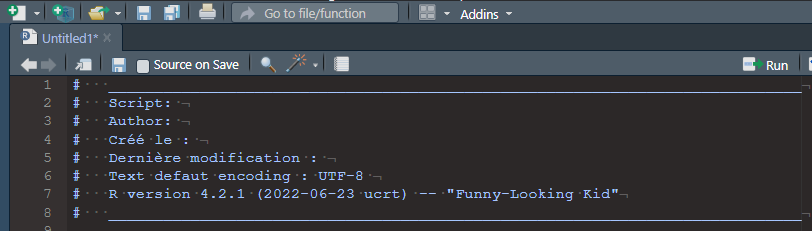
\includegraphics[width=0.3\linewidth,height=\textheight,keepaspectratio]{img/screenshot_RStudio_EnTeteScript.png}
\end{center}

\begin{enumerate}
\def\labelenumi{\arabic{enumi}.}
\setcounter{enumi}{1}
\tightlist
\item
  Ajouter la \textbf{liste des packages utilisés} et leur version
\end{enumerate}

\begin{enumerate}
\def\labelenumi{\arabic{enumi}.}
\setcounter{enumi}{2}
\tightlist
\item
  \textbf{Structurer} en parties et sous-parties grâce à l'\emph{addin}
  \texttt{strcode}\\
  
\includegraphics[width=1.25em,height=1em]{index_files/figure-pdf/fa-icon-6e3e6b566131db41246b1ca486a392da.pdf}
  \emph{\texttt{remotes::install\_github("lorenzwalthert/strcode")}}
\end{enumerate}

\begin{Shaded}
\begin{Highlighting}[]
\CommentTok{\#   \_\_\_\_\_\_\_\_\_\_\_\_\_\_\_\_\_\_\_\_\_\_\_\_\_\_\_\_\_\_\_\_\_\_\_\_\_\_\_\_\_\_\_\_}
\CommentTok{\#   Titre 1                                 \#\#\#\#}
\DocumentationTok{\#\#  ............................................}
\DocumentationTok{\#\#  Titre 2                                 \#\#\#\#}
\end{Highlighting}
\end{Shaded}

\begin{enumerate}
\def\labelenumi{\arabic{enumi}.}
\setcounter{enumi}{3}
\tightlist
\item
  Commenter les scripts (avec le signe \texttt{\#}), en particulier pour
  expliquer les étapes-clés
\end{enumerate}

\begin{tcolorbox}[enhanced jigsaw, arc=.35mm, bottomrule=.15mm, bottomtitle=1mm, breakable, colback=white, colbacktitle=quarto-callout-tip-color!10!white, colframe=quarto-callout-tip-color-frame, coltitle=black, left=2mm, leftrule=.75mm, opacityback=0, opacitybacktitle=0.6, rightrule=.15mm, title=\textcolor{quarto-callout-tip-color}{\faLightbulb}\hspace{0.5em}{Comment passer une ligne entière en commentaires ?}, titlerule=0mm, toprule=.15mm, toptitle=1mm]


\includegraphics[width=0.75em,height=1em]{index_files/figure-pdf/fa-icon-04c6f9870c69c7270c705a206c46d917.pdf}
\textbf{Avec un raccourci clavier} : se placer sur la ligne et cliquer
sur \texttt{CRTL\ +\ MAJ\ +\ C}

\end{tcolorbox}

\begin{center}\rule{0.5\linewidth}{0.5pt}\end{center}

\begin{tcolorbox}[enhanced jigsaw, arc=.35mm, bottomrule=.15mm, bottomtitle=1mm, breakable, colback=white, colbacktitle=quarto-callout-note-color!10!white, colframe=quarto-callout-note-color-frame, coltitle=black, left=2mm, leftrule=.75mm, opacityback=0, opacitybacktitle=0.6, rightrule=.15mm, title=\textcolor{quarto-callout-note-color}{\faInfo}\hspace{0.5em}{Respecter des règles pour faciliter la lecture}, titlerule=0mm, toprule=.15mm, toptitle=1mm]

\begin{itemize}
\tightlist
\item
  Retour à la ligne régulièrement (\textbf{la longueur maximale
  recommandée d'une ligne est 80 caractères}) et après chaque pipe
  (\texttt{\%\textgreater{}\%} ou \texttt{\textbar{}\textgreater{}})\\
\item
  L'indentation se fait grâce à la touche \texttt{TAB}. Le raccourci
  \texttt{Ctrl+I} sert à réindenter les lignes de code sélectionnées\\
\item
  Les opérateurs qui lient les objets entre eux
  \texttt{(=,\ +,\ -,\ \textless{}-,\ etc.)} sont entourés d'espaces\\
\item
  Les opérateurs qui modifient un objet ou sélectionnent une partie d'un
  objet \texttt{(:,\ !!,\ \$,\ @,\ {[},\ {]},\ {[}{[},\ {]}{]})} ne sont
  pas entourés d'espaces
\end{itemize}

\begin{Shaded}
\begin{Highlighting}[]
\CommentTok{\# On écrit }
\DecValTok{1} \SpecialCharTok{+} \DecValTok{1} \OtherTok{=} \DecValTok{2}
\NormalTok{dataframe}\SpecialCharTok{$}\NormalTok{variable}
\end{Highlighting}
\end{Shaded}

\begin{Shaded}
\begin{Highlighting}[]
\CommentTok{\# et non }
\DecValTok{1}\SpecialCharTok{+}\DecValTok{1}\OtherTok{=}\DecValTok{2}
\NormalTok{dataframe }\SpecialCharTok{$}\NormalTok{ variable}
\end{Highlighting}
\end{Shaded}

\begin{itemize}
\tightlist
\item
  On insère un espace après la virgule mais pas avant, comme en français
  !\\
\item
  On ne met pas d'espace avant ou après les parenthèses\\
\item
  En revanche, les opérateurs de comparaison doivent être entourés
  d'espace pour ne pas être mal interprétés par \textbf{R}
\end{itemize}

\begin{Shaded}
\begin{Highlighting}[]
\CommentTok{\# On écrit}
\FunctionTok{mean}\NormalTok{(x, }\AttributeTok{na.rm =} \ConstantTok{TRUE}\NormalTok{)  }
\DecValTok{1} \SpecialCharTok{\textless{}} \SpecialCharTok{{-}}\DecValTok{10}
\end{Highlighting}
\end{Shaded}

\begin{Shaded}
\begin{Highlighting}[]
\CommentTok{\# et non }
\FunctionTok{mean}\NormalTok{ ( x , }\AttributeTok{na.rm =} \ConstantTok{TRUE}\NormalTok{ )}
\DecValTok{1}\OtherTok{\textless{}{-}}\DecValTok{10}
\end{Highlighting}
\end{Shaded}

\end{tcolorbox}

\begin{center}\rule{0.5\linewidth}{0.5pt}\end{center}

\begin{tcolorbox}[enhanced jigsaw, arc=.35mm, bottomrule=.15mm, bottomtitle=1mm, breakable, colback=white, colbacktitle=quarto-callout-tip-color!10!white, colframe=quarto-callout-tip-color-frame, coltitle=black, left=2mm, leftrule=.75mm, opacityback=0, opacitybacktitle=0.6, rightrule=.15mm, title=\textcolor{quarto-callout-tip-color}{\faLightbulb}\hspace{0.5em}{Aide pour écrire les scripts}, titlerule=0mm, toprule=.15mm, toptitle=1mm]


\includegraphics[width=1.25em,height=1em]{index_files/figure-pdf/fa-icon-6e3e6b566131db41246b1ca486a392da.pdf}
Activer les options de diagnostic pour que \textbf{RStudio} signale
automatiquement les erreurs dans les scripts :
\texttt{Tools\ \textgreater{}\ Global\ Options\ \textgreater{}\ Code\ \textgreater{}\ Diagnostics}

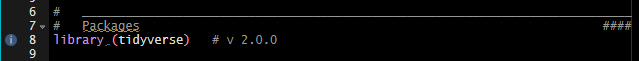
\includegraphics[width=1\linewidth,height=\textheight,keepaspectratio]{img/screenshot_diagnostic_script.png}


\includegraphics[width=1.13em,height=1em]{index_files/figure-pdf/fa-icon-8efa9b48ef60e317e1d84ab04f11b153.pdf}
package \href{https://github.com/r-lib/styler}{\{styler\}} : mettre en
forme le code selon le
\href{https://style.tidyverse.org/index.html}{Tidyverse Style Guide} (ou
selon son propre style)


\includegraphics[width=1.13em,height=1em]{index_files/figure-pdf/fa-icon-8efa9b48ef60e317e1d84ab04f11b153.pdf}
package \href{https://lintr.r-lib.org/}{\{lintr\}} : vérifier que le
code est conforme à un guide de style donné

\end{tcolorbox}

\begin{center}\rule{0.5\linewidth}{0.5pt}\end{center}

\begin{tcolorbox}[enhanced jigsaw, arc=.35mm, bottomrule=.15mm, bottomtitle=1mm, breakable, colback=white, colbacktitle=quarto-callout-tip-color!10!white, colframe=quarto-callout-tip-color-frame, coltitle=black, left=2mm, leftrule=.75mm, opacityback=0, opacitybacktitle=0.6, rightrule=.15mm, title=\textcolor{quarto-callout-tip-color}{\faLightbulb}\hspace{0.5em}{Le fichier README}, titlerule=0mm, toprule=.15mm, toptitle=1mm]

Il est recommandé de créer un fichier README, dans le dossier du projet,
qui présente le \textbf{projet}, sa \textbf{structuration} et les
\textbf{étapes d'exécution des différents script} pour comprendre,
reproduire et utiliser le projet


\includegraphics[width=0.75em,height=1em]{index_files/figure-pdf/fa-icon-04c6f9870c69c7270c705a206c46d917.pdf}
\textbf{Un README est généralement un fichier au format .txt ou .md
(markdown)}

\textbf{Exemple de fichier README}

\begin{Shaded}
\begin{Highlighting}[]
\NormalTok{\# BulleR}

\NormalTok{Projet de la session}

\NormalTok{\#\# Structure}
\NormalTok{{-} data/ : données }
\NormalTok{    ├── sources/ : données sources, données brutes}
\NormalTok{    └── produites/ : données produites}
\NormalTok{{-} scripts/ : scripts R, qmd}
\NormalTok{{-} outputs/ : graphiques et tableaux exportés}
\NormalTok{{-} docs/ : rapports et supports}

\NormalTok{\#\# Comment reproduire les analyses}
\NormalTok{1. Ouvrir le projet \textasciigrave{}BulleR\textasciigrave{}}
\NormalTok{2. Exécuter les scripts dans l\textquotesingle{}ordre (01\_import.R, 02\_nettoyage.R, etc.)}
\NormalTok{3. Les graphiques générés sont enregistrés dans le dossier outputs}
\NormalTok{4. Le rapport d\textquotesingle{}étude est enregistré dans le dossier docs}
\end{Highlighting}
\end{Shaded}

\end{tcolorbox}

\section{\texorpdfstring{Introduction au
\texttt{tidyverse}}{Introduction au tidyverse}}\label{introduction-au-tidyverse}

\subsection{\texorpdfstring{\textbf{R} vs
\texttt{tidyverse}}{R vs tidyverse}}\label{r-vs-tidyverse}

\begin{itemize}
\tightlist
\item
  Deux ``façons'' d'écrire du \textbf{R}
\item
  Mêmes résultats, styles différents
\end{itemize}

\subsubsection{\texorpdfstring{\textbf{R} de
base}{R de base}}\label{r-de-base}

\begin{itemize}
\tightlist
\item
  Fonctions et syntaxe incluses dans \textbf{R}
\item
  Syntaxe parfois hétérogène
\item
  Beaucoup d'opérateurs spéciaux pour manipuler les données :
  \texttt{{[}}, \texttt{{[}{[}}, \texttt{\$}, \texttt{which()},
  \texttt{apply()}, etc.
\item
  Les fonctions s'imbriquent, création de nombreux objets intermédiaires
\item
  Code souvent ``compact'', mais parfois difficile à lire pour les
  débutants
\end{itemize}

\emph{Exemple}

\begin{Shaded}
\begin{Highlighting}[]
\NormalTok{res }\OtherTok{\textless{}{-}} \FunctionTok{head}\NormalTok{(}\FunctionTok{subset}\NormalTok{(Journals, citestot }\SpecialCharTok{\textgreater{}} \DecValTok{20}\NormalTok{))}
\CommentTok{\# ou}
\NormalTok{tmp }\OtherTok{\textless{}{-}}\NormalTok{ Journals[Journals}\SpecialCharTok{$}\NormalTok{citestot }\SpecialCharTok{\textgreater{}} \DecValTok{20}\NormalTok{, ]}
\NormalTok{res }\OtherTok{\textless{}{-}} \FunctionTok{head}\NormalTok{(tmp)}
\end{Highlighting}
\end{Shaded}

\subsubsection{tidyverse}\label{tidyverse}

\begin{itemize}
\tightlist
\item
  Ensemble de packages qui reprennent des opérations courantes de
  \textbf{R} de façon unifiée, conçus pour travailler ensemble

  \begin{itemize}
  \tightlist
  \item
    uniformité des formats d'entrée et de sortie
  \item
    syntaxe commune entre les packages
  \item
    les noms de fonctions sont des verbes : \texttt{filter()},
    \texttt{select()}, \texttt{mutate()}, \texttt{summarise()},
    \texttt{arrange()}, \texttt{join()}
  \end{itemize}
\item
  Philosophie ``tidy'' : données en tables ``propres'', fonctions
  cohérentes, code lisible
\item
  L'accent est mis sur la lisibilité et la chaîne d'opérations, via
  l'opérateur \emph{pipe} \texttt{\textbar{}\textgreater{}}\\
  \(\Rightarrow\) le code suit l'ordre logique des étapes, avec moins
  d'objets intermédiaires, moins de parenthèses imbriquées
\end{itemize}

\emph{Exemple}

\begin{Shaded}
\begin{Highlighting}[]
\FunctionTok{library}\NormalTok{(dplyr)}

\NormalTok{Journals }\SpecialCharTok{|\textgreater{}} 
  \FunctionTok{filter}\NormalTok{(citestot }\SpecialCharTok{\textgreater{}} \DecValTok{20}\NormalTok{) }\SpecialCharTok{|\textgreater{}} 
  \FunctionTok{head}\NormalTok{()}
\end{Highlighting}
\end{Shaded}

\begin{center}\rule{0.5\linewidth}{0.5pt}\end{center}

\paragraph{\texorpdfstring{L'opérateur
\emph{pipe}}{L'opérateur pipe}}\label{lopuxe9rateur-pipe}

\begin{itemize}
\tightlist
\item
  Opérateur qui permet d'enchaîner des opérations : il prend la sortie
  d'une fonction (ou d'une expression) et la passe automatiquement comme
  \textbf{premier} argument à la fonction suivante
\item
  Initialement fourni dans le package
  \href{https://magrittr.tidyverse.org/}{\{magrittr\}} et noté
  \texttt{\%\textgreater{}\%}
\item
  Implémenté dans le langage \textbf{R} de base depuis la version 4.1.0
  et noté \texttt{\textbar{}\textgreater{}}
\end{itemize}

\begin{Shaded}
\begin{Highlighting}[]
\NormalTok{data }\SpecialCharTok{|\textgreater{}}
  \FunctionTok{fonction1}\NormalTok{() }\SpecialCharTok{|\textgreater{}}
  \FunctionTok{fonction2}\NormalTok{() }\SpecialCharTok{|\textgreater{}}
  \FunctionTok{fonction3}\NormalTok{()}
\CommentTok{\# équivaut à}
\FunctionTok{fonction3}\NormalTok{(}\FunctionTok{fonction2}\NormalTok{(}\FunctionTok{fonction1}\NormalTok{(data)))}
\end{Highlighting}
\end{Shaded}

\begin{tcolorbox}[enhanced jigsaw, arc=.35mm, bottomrule=.15mm, breakable, colback=white, colframe=quarto-callout-tip-color-frame, left=2mm, leftrule=.75mm, opacityback=0, rightrule=.15mm, toprule=.15mm]
\begin{minipage}[t]{5.5mm}
\textcolor{quarto-callout-tip-color}{\faLightbulb}
\end{minipage}%
\begin{minipage}[t]{\textwidth - 5.5mm}

\textbf{Il est recommandé d'utiliser le pipe natif de R}
\texttt{\textbar{}\textgreater{}}


\includegraphics[width=1.25em,height=1em]{index_files/figure-pdf/fa-icon-6e3e6b566131db41246b1ca486a392da.pdf}
\textbf{Comment utiliser le pipe natif sous RStudio ?}\\
- Allez dans
\texttt{Tools\ \textgreater{}\ Global\ Options\ \textgreater{}\ Code\ \textgreater{}\ Editing}\\
- Cochez
\texttt{Use\ native\ pipe\ operator,\ \textbar{}\textgreater{}\ (requires\ R\ 4.1+)}

\end{minipage}%
\end{tcolorbox}

\begin{center}\rule{0.5\linewidth}{0.5pt}\end{center}

\paragraph{\texorpdfstring{Les
\emph{tibbles}}{Les tibbles}}\label{les-tibbles}

\begin{itemize}
\tightlist
\item
  \textbf{Version modernisée des \emph{dataframes}}, proposée dans le
  cadre du \texttt{tidyverse}
\item
  Plus pratiques à utiliser que les \emph{dataframes} ``classiques''
\item
  Plus rapides à manipuler (et plus stables) que les \emph{dataframes}
\item
  Il est possible de convertir d'un type à l'autre

  \begin{itemize}
  \tightlist
  \item
    \emph{dataframe} \(\rightarrow\) \emph{tibble} : avec la fonction
    \texttt{as\_tibble()} du package
    \href{https://tibble.tidyverse.org/}{\{tibble\}}\\
  \item
    \emph{tibble} \(\rightarrow\) \emph{dataframe} : avec la fonction
    \textbf{R} de base \texttt{as.data.frame()}
  \end{itemize}
\end{itemize}

\begin{center}\rule{0.5\linewidth}{0.5pt}\end{center}

\begin{tcolorbox}[enhanced jigsaw, arc=.35mm, bottomrule=.15mm, bottomtitle=1mm, breakable, colback=white, colbacktitle=quarto-callout-note-color!10!white, colframe=quarto-callout-note-color-frame, coltitle=black, left=2mm, leftrule=.75mm, opacityback=0, opacitybacktitle=0.6, rightrule=.15mm, title=\textcolor{quarto-callout-note-color}{\faInfo}\hspace{0.5em}{Aperçu des formats}, titlerule=0mm, toprule=.15mm, toptitle=1mm]

\textbf{\emph{dataframe}}

\begin{Shaded}
\begin{Highlighting}[]
\NormalTok{Journals }\SpecialCharTok{|\textgreater{}} 
  \FunctionTok{head}\NormalTok{(}\DecValTok{2}\NormalTok{)}
\end{Highlighting}
\end{Shaded}

\begin{verbatim}
                                      title                    pub society libprice pages charpp citestot date1 oclc      field
1         Asian-Pacific Economic Literature              Blackwell      no      123   440   3822       21  1986   14    General
2 South African Journal of Economic History So Afr ec history assn      no       20   309   1782       22  1986   59 Ec History
\end{verbatim}

\textbf{\emph{tibble}}

\begin{Shaded}
\begin{Highlighting}[]
\NormalTok{Journals }\SpecialCharTok{|\textgreater{}} 
  \FunctionTok{as\_tibble}\NormalTok{() }\SpecialCharTok{|\textgreater{}} 
  \FunctionTok{head}\NormalTok{(}\DecValTok{2}\NormalTok{)}
\end{Highlighting}
\end{Shaded}

\begin{verbatim}
# A tibble: 2 x 10
  title                                     pub                    society libprice pages charpp citestot date1  oclc field     
  <fct>                                     <fct>                  <fct>      <int> <int>  <int>    <int> <int> <int> <fct>     
1 Asian-Pacific Economic Literature         Blackwell              no           123   440   3822       21  1986    14 General   
2 South African Journal of Economic History So Afr ec history assn no            20   309   1782       22  1986    59 Ec History
\end{verbatim}

\end{tcolorbox}

\subsection{\texorpdfstring{Installation du
\texttt{tidyverse}}{Installation du tidyverse}}\label{installation-du-tidyverse}

\begin{itemize}
\item
  
\includegraphics[width=1.25em,height=1em]{index_files/figure-pdf/fa-icon-6e3e6b566131db41246b1ca486a392da.pdf}
  La commande \texttt{install.packages("tidyverse")} installe
  simultanément plusieurs packages

  \begin{itemize}
  \tightlist
  \item
    \href{https://dplyr.tidyverse.org/}{\{dplyr\}} : manipulation des
    données
  \item
    \href{https://forcats.tidyverse.org/}{\{forcats\}} : traitement des
    variables qualitatives
  \item
    \href{https://ggplot2.tidyverse.org/}{\{ggplot2\}} : visualisation
    des données
  \item
    \href{https://lubridate.tidyverse.org/}{\{lubridate\}} :
    manipulation des dates et heures
  \item
    \href{https://purrr.tidyverse.org/}{\{purrr\}} : programmation
  \item
    \href{https://readr.tidyverse.org/}{\{readr\}} : import de données
  \item
    \href{https://stringr.tidyverse.org/}{\{stringr\}} : manipulation
    des chaînes de caractères
  \item
    \href{https://tibble.tidyverse.org/}{\{tibble\}} : version
    modernisée des \emph{dataframes}, plus pratiques à utiliser que les
    \emph{dataframes} ``classiques''
  \item
    \href{https://tidyr.tidyverse.org/}{\{tidyr\}} : nettoyage, remise
    en forme des données
  \end{itemize}
\end{itemize}

\begin{center}\rule{0.5\linewidth}{0.5pt}\end{center}

\subsubsection{\texorpdfstring{Les packages du \texttt{tidyverse} dans
la \emph{Data
Science}}{Les packages du tidyverse dans la Data Science}}\label{les-packages-du-tidyverse-dans-la-data-science}

\begin{center}
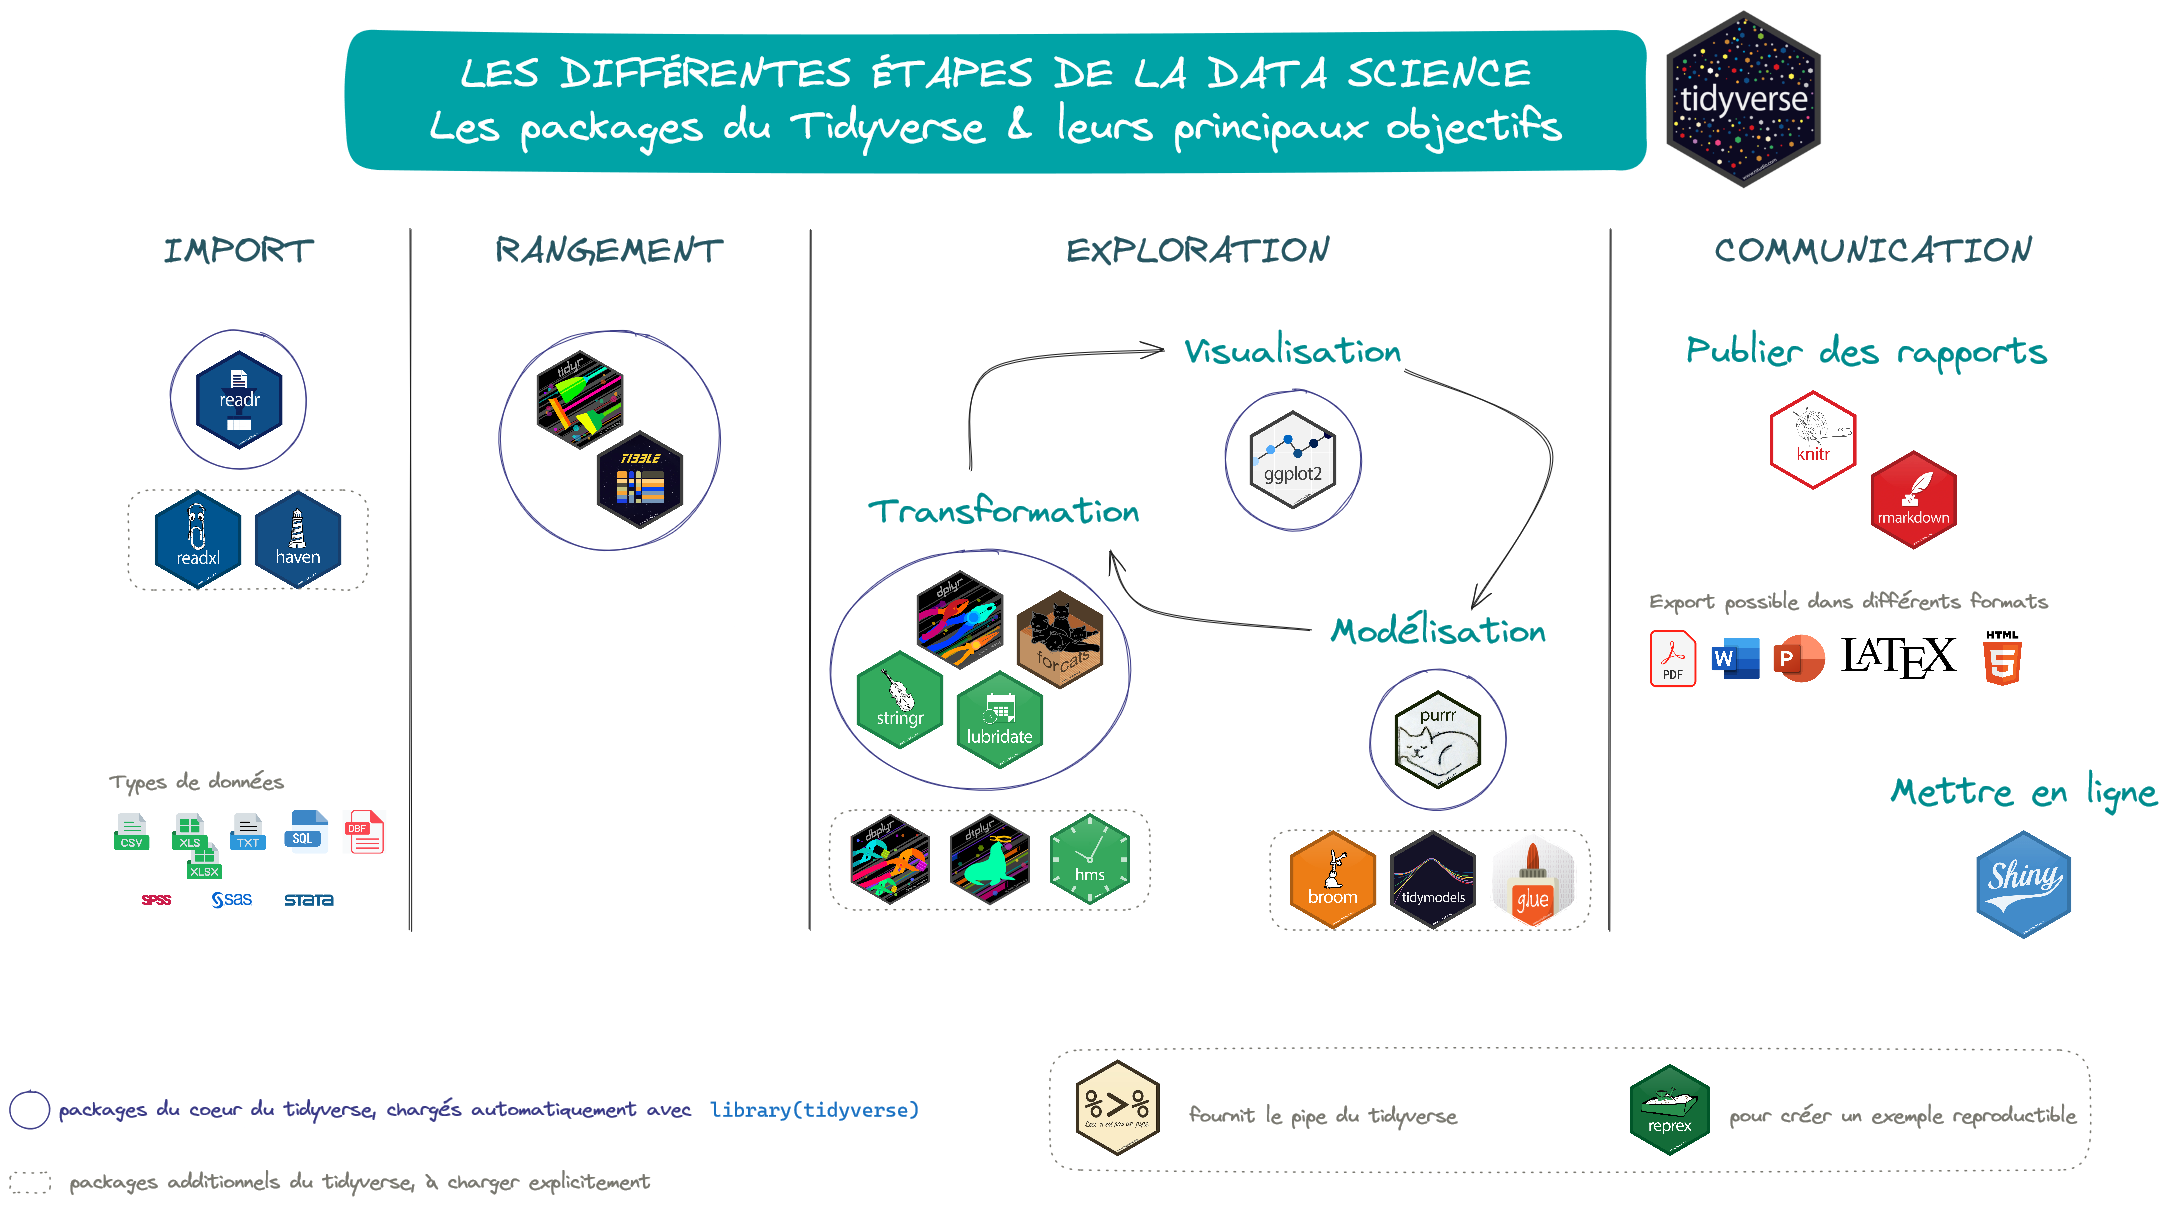
\includegraphics[width=0.8\linewidth,height=\textheight,keepaspectratio]{img/tidyverse_workflow_2024.png}
\end{center}

\section{Premières manipulations}\label{premiuxe8res-manipulations}

\subsection{Import/Export des
données}\label{importexport-des-donnuxe9es}

\begin{itemize}
\tightlist
\item
  Depuis/vers des formats ``plats'' ou délimités (.csv, .txt)
\item
  Depuis/vers des fichiers Excel ou issus d'autres logiciels de
  statistique (Stata, SPSS, etc.)
\item
  Depuis/vers des bases de données relationnelles
\end{itemize}

\begin{tcolorbox}[enhanced jigsaw, arc=.35mm, bottomrule=.15mm, bottomtitle=1mm, breakable, colback=white, colbacktitle=quarto-callout-tip-color!10!white, colframe=quarto-callout-tip-color-frame, coltitle=black, left=2mm, leftrule=.75mm, opacityback=0, opacitybacktitle=0.6, rightrule=.15mm, title=\textcolor{quarto-callout-tip-color}{\faLightbulb}\hspace{0.5em}{Pour l'import, bien étudier le jeu de données source, à l'aide des
questions suivantes}, titlerule=0mm, toprule=.15mm, toptitle=1mm]

\begin{enumerate}
\def\labelenumi{\arabic{enumi}.}
\tightlist
\item
  La première ligne contient-elle le nom des variables ?\\
\item
  Quel est le séparateur des colonnes : \texttt{,}, \texttt{;},
  espace(s), \texttt{\textbackslash{}t} ?\\
\item
  Quel est le caractère utilisé pour indiquer les décimales : le point
  (à l'anglo-saxonne) ou la virgule (à la française) ?\\
\item
  Les valeurs textuelles sont-elles encadrées par des guillemets ? Si
  oui, s'agit-il de guillemets simples (\texttt{\textquotesingle{}}) ou
  de guillemets doubles (\texttt{"}) ?\\
\item
  Y a-t-il des valeurs manquantes ? Si oui, comment sont-elles indiquées
  ?\\
\end{enumerate}

\end{tcolorbox}

\subsubsection{Les fonctions d'import}\label{les-fonctions-dimport}

{\def\LTcaptype{none} % do not increment counter
\begin{longtable}[]{@{}
  >{\raggedright\arraybackslash}p{(\linewidth - 8\tabcolsep) * \real{0.1000}}
  >{\raggedright\arraybackslash}p{(\linewidth - 8\tabcolsep) * \real{0.2000}}
  >{\raggedright\arraybackslash}p{(\linewidth - 8\tabcolsep) * \real{0.2000}}
  >{\raggedright\arraybackslash}p{(\linewidth - 8\tabcolsep) * \real{0.2500}}
  >{\raggedright\arraybackslash}p{(\linewidth - 8\tabcolsep) * \real{0.2500}}@{}}
\toprule\noalign{}
\begin{minipage}[b]{\linewidth}\raggedright
Type de fichier
\end{minipage} & \begin{minipage}[b]{\linewidth}\raggedright
Séparateur de colonnes
\end{minipage} & \begin{minipage}[b]{\linewidth}\raggedright
Séparateur décimal
\end{minipage} & \begin{minipage}[b]{\linewidth}\raggedright
Tidyverse
\end{minipage} & \begin{minipage}[b]{\linewidth}\raggedright
Base R
\end{minipage} \\
\midrule\noalign{}
\endhead
\bottomrule\noalign{}
\endlastfoot
Délimité & \texttt{,} & \texttt{.} & \texttt{readr::read\_csv()} &
\texttt{read.csv()} \\
& \texttt{;} & \texttt{,} & \texttt{readr::read\_csv2()} &
\texttt{read.csv2()} \\
& un espace (ou plus) & \texttt{.} & \texttt{readr::read\_table()} &
\texttt{read.table()} \\
& \texttt{\textbackslash{}t} & \texttt{.} &
\texttt{readr::read\_delim()} & \texttt{read.delim()} \\
& \texttt{\textbackslash{}t} & \texttt{,} &
\texttt{readr::read\_delim2()} & \texttt{read.delim2()} \\
Excel & & & \texttt{readxl::read\_excel()} &
\texttt{xlsx::read.xlsx()} \\
SPSS & & & \texttt{haven::read\_spss()} &
\texttt{foreign::read.spss()} \\
& & & \texttt{haven::read\_sav()} & \\
Stata & & & \texttt{haven::read\_stata()} &
\texttt{foreign::read.dta()} \\
SAS & & & \texttt{haven::read\_sas()} & \texttt{foreign::read.ssd()} \\
dBase & & & & \texttt{foreign::read.dbf()} \\
\end{longtable}
}

\subsubsection{Les fonctions d'export}\label{les-fonctions-dexport}

{\def\LTcaptype{none} % do not increment counter
\begin{longtable}[]{@{}
  >{\raggedright\arraybackslash}p{(\linewidth - 4\tabcolsep) * \real{0.1753}}
  >{\raggedright\arraybackslash}p{(\linewidth - 4\tabcolsep) * \real{0.3711}}
  >{\raggedright\arraybackslash}p{(\linewidth - 4\tabcolsep) * \real{0.4536}}@{}}
\toprule\noalign{}
\begin{minipage}[b]{\linewidth}\raggedright
Type de fichier
\end{minipage} & \begin{minipage}[b]{\linewidth}\raggedright
Tidyverse
\end{minipage} & \begin{minipage}[b]{\linewidth}\raggedright
Base R
\end{minipage} \\
\midrule\noalign{}
\endhead
\bottomrule\noalign{}
\endlastfoot
.txt & \texttt{readr::write\_delim(delim\ =\ "\textbackslash{}t")} &
\texttt{write.table()} \\
.csv & \texttt{readr::write\_csv()} & \texttt{write.csv()} \\
.xlsx & \texttt{openxlsx2::write\_xlsx()} & \\
& \texttt{writexl::write\_xlsx()} & \\
.dbf & & \texttt{foreign::write.dbf()} \\
.sav (SPSS) & \texttt{haven::write\_sav()} &
\texttt{foreign::write.foreign(package\ =\ "SPSS")} \\
.dta (Stata) & \texttt{haven::write\_dta()} &
\texttt{foreign::write.dta()} \\
\end{longtable}
}

\begin{center}\rule{0.5\linewidth}{0.5pt}\end{center}

\subparagraph{Exemple d'import pour un fichier
.csv}\label{exemple-dimport-pour-un-fichier-.csv}

\begin{Shaded}
\begin{Highlighting}[]
\NormalTok{readr}\SpecialCharTok{::}\FunctionTok{read\_csv}\NormalTok{(}\StringTok{"file.csv"}
                \CommentTok{\# si la première ligne contient le nom des variables :}
\NormalTok{                , }\AttributeTok{col\_names =} \ConstantTok{TRUE}\NormalTok{)}
\end{Highlighting}
\end{Shaded}

\begin{tcolorbox}[enhanced jigsaw, arc=.35mm, bottomrule=.15mm, bottomtitle=1mm, breakable, colback=white, colbacktitle=quarto-callout-tip-color!10!white, colframe=quarto-callout-tip-color-frame, coltitle=black, left=2mm, leftrule=.75mm, opacityback=0, opacitybacktitle=0.6, rightrule=.15mm, title=\textcolor{quarto-callout-tip-color}{\faLightbulb}\hspace{0.5em}{Zoom sur la fonction \texttt{read\_csv2()}}, titlerule=0mm, toprule=.15mm, toptitle=1mm]

La fonction \texttt{readr::read\_csv2()} considère par défaut que le
séparateur de colonnes est le point-virgule et que la virgule sert de
séparateur décimal

La fonction en langage {R} de base \texttt{read.csv2()} a les mêmes
paramètres par défaut


\includegraphics[width=0.75em,height=1em]{index_files/figure-pdf/fa-icon-04c6f9870c69c7270c705a206c46d917.pdf}
\textbf{Utiliser ces fonctions lorsque les fichiers .csv ont ces
caractéristiques}

\end{tcolorbox}

\subsection{Manipulations sur les données avec le package
\{dplyr\}}\label{manipulations-sur-les-donnuxe9es-avec-le-package-dplyr}

\subsubsection{\texorpdfstring{Sélection de lignes avec la fonction
\texttt{filter()}}{Sélection de lignes avec la fonction filter()}}\label{suxe9lection-de-lignes-avec-la-fonction-filter}

\begin{Shaded}
\begin{Highlighting}[]
\CommentTok{\# Revues dans le domaine de la Démographie}
\NormalTok{Journals }\SpecialCharTok{|\textgreater{}}
\NormalTok{  dplyr}\SpecialCharTok{::}\FunctionTok{filter}\NormalTok{(field }\SpecialCharTok{==} \StringTok{"Demography"}\NormalTok{)}
\end{Highlighting}
\end{Shaded}

\begin{verbatim}
                              title                pub society libprice pages charpp citestot date1 oclc      field
30  Journal of Population Economics           Springer      no      411   640   3264       69  1987   27 Demography
116 Population & Development Review Population Council      no       36   910   2904      445  1975  218 Demography
137                      Demography   Pop Assn America      no       85   568   6859      670  1964  413 Demography
\end{verbatim}

\subsubsection{\texorpdfstring{Sélection de colonnes avec la fonction
\texttt{select()}}{Sélection de colonnes avec la fonction select()}}\label{suxe9lection-de-colonnes-avec-la-fonction-select}

\begin{Shaded}
\begin{Highlighting}[]
\CommentTok{\# Sélection de la variable "pub"}
\NormalTok{Journals }\SpecialCharTok{|\textgreater{}}
\NormalTok{  dplyr}\SpecialCharTok{::}\FunctionTok{select}\NormalTok{(pub)}
\end{Highlighting}
\end{Shaded}

\begin{verbatim}
                            pub
1                     Blackwell
2        So Afr ec history assn
3                        Kluwer
4                        Kluwer
5                      Elsevier
6                      Elsevier
7           Cambridge Univ Pres
8                      Elsevier
9                        Kluwer
...
\end{verbatim}

\subsubsection{\texorpdfstring{Création de nouvelles variables avec la
fonction
\texttt{mutate()}}{Création de nouvelles variables avec la fonction mutate()}}\label{cruxe9ation-de-nouvelles-variables-avec-la-fonction-mutate}

\begin{Shaded}
\begin{Highlighting}[]
\CommentTok{\# Ajout de la variable "anciennete"}
\NormalTok{Journals }\SpecialCharTok{|\textgreater{}}
  \FunctionTok{mutate}\NormalTok{(}\AttributeTok{anciennete =} \DecValTok{2025} \SpecialCharTok{{-}}\NormalTok{ date1) }\OtherTok{{-}\textgreater{}}\NormalTok{ Journals}

\FunctionTok{names}\NormalTok{(Journals)}
\end{Highlighting}
\end{Shaded}

\begin{verbatim}
 [1] "title"      "pub"        "society"    "libprice"   "pages"      "charpp"     "citestot"   "date1"     
 [9] "oclc"       "field"      "anciennete"
\end{verbatim}


\includegraphics[width=0.75em,height=1em]{index_files/figure-pdf/fa-icon-04c6f9870c69c7270c705a206c46d917.pdf}
\textbf{Penser à affecter le résultat à un objet si nécessaire !}

\subsection{Besoin d'examiner rapidement vos données dans Excel
?}\label{besoin-dexaminer-rapidement-vos-donnuxe9es-dans-excel}

Utilisez l'addin \texttt{viewxl} pour exporter interactivement les
\emph{dataframes} de l'environnement \textbf{R} vers Excel

\begin{itemize}
\tightlist
\item
  via le menu
  \texttt{Addins\ \textgreater{}\ VIEWXL\ \textgreater{}\ View\ in\ Excel}
\end{itemize}

\begin{center}
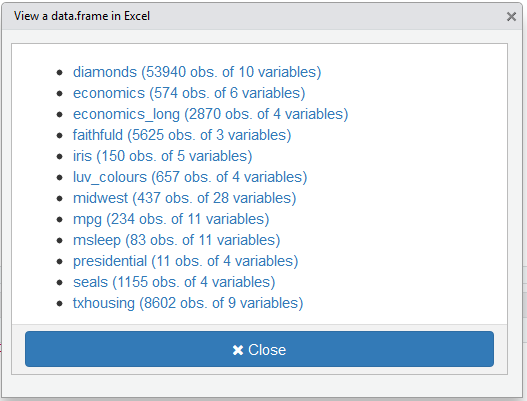
\includegraphics[width=0.7\linewidth,height=\textheight,keepaspectratio]{img/viewxl.png}
\end{center}

\begin{itemize}
\tightlist
\item
  dans la console, avec la fonction \texttt{view\_in\_xl()} :
\end{itemize}

\begin{Shaded}
\begin{Highlighting}[]
\NormalTok{viewxl}\SpecialCharTok{::}\FunctionTok{view\_in\_xl}\NormalTok{(diamonds)}
\end{Highlighting}
\end{Shaded}

\begin{tcolorbox}[enhanced jigsaw, arc=.35mm, bottomrule=.15mm, breakable, colback=white, colframe=quarto-callout-warning-color-frame, left=2mm, leftrule=.75mm, opacityback=0, rightrule=.15mm, toprule=.15mm]
\begin{minipage}[t]{5.5mm}
\textcolor{quarto-callout-warning-color}{\faExclamationTriangle}
\end{minipage}%
\begin{minipage}[t]{\textwidth - 5.5mm}

\textbf{\texttt{viewxl} ne sert qu'à visualiser les données sous Excel,
et non pas à faire des modifications sur les données. Les modifications
se font toujours sur R !}

\end{minipage}%
\end{tcolorbox}

\section{Pour conclure}\label{pour-conclure}

\subsection{\texorpdfstring{De nombreuses ressources pour faciliter
l'usage de
\textbf{R}}{De nombreuses ressources pour faciliter l'usage de R}}\label{de-nombreuses-ressources-pour-faciliter-lusage-de-r}

\subsubsection{\texorpdfstring{Des packages et/ou
\href{https://github.com/daattali/addinslist}{\emph{addins}}
(extensions)}{Des packages et/ou addins (extensions)}}\label{des-packages-etou-addins-extensions}


\includegraphics[width=1.13em,height=1em]{index_files/figure-pdf/fa-icon-8efa9b48ef60e317e1d84ab04f11b153.pdf}
\href{https://github.com/daattali/addinslist}{\{addinslist\}} :
parcourir et installer les \emph{addins} de \textbf{RStudio}


\includegraphics[width=1.13em,height=1em]{index_files/figure-pdf/fa-icon-8efa9b48ef60e317e1d84ab04f11b153.pdf}
\href{https://juba.github.io/questionr/}{\{questionr\}} : manipuler,
recoder, nettoyer et analyser (tableaux de fréquence par exemple) des
données d'enquêtes (par questionnaire)


\includegraphics[width=1.13em,height=1em]{index_files/figure-pdf/fa-icon-8efa9b48ef60e317e1d84ab04f11b153.pdf}
\href{https://github.com/skranz/ReplaceInFiles}{\{ReplaceInFiles\}} :
rechercher et remplacer une valeur dans plusieurs fichiers


\includegraphics[width=1.13em,height=1em]{index_files/figure-pdf/fa-icon-8efa9b48ef60e317e1d84ab04f11b153.pdf}
\href{https://lorenzwalthert.github.io/strcode}{\{strcode\}} :
structurer le code (sauts de section avec titre en en-tête)

\subsubsection{Des ressources en ligne}\label{des-ressources-en-ligne}


\includegraphics[width=1em,height=1em]{index_files/figure-pdf/fa-icon-be1da9f9a11cb30d6d0a10a027b462cd.pdf}
Sur le CRAN, des \href{https://cran.r-project.org/manuals.html}{manuels}
et d'\href{https://cran.r-project.org/other-docs.html}{autres
contributions}


\includegraphics[width=1em,height=1em]{index_files/figure-pdf/fa-icon-be1da9f9a11cb30d6d0a10a027b462cd.pdf}
\href{http://www.r-project.org}{R project}


\includegraphics[width=1em,height=1em]{index_files/figure-pdf/fa-icon-be1da9f9a11cb30d6d0a10a027b462cd.pdf}
\href{http://www.rseek.org}{Rseek} : moteur de recherche dédié à
\textbf{R}


\includegraphics[width=0.88em,height=1em]{index_files/figure-pdf/fa-icon-9db699512b3663cebc4c654768f9dd87.pdf}
Des \href{https://rstudio.com/resources/cheatsheets}{\emph{cheatsheets}}
(fiches synthétiques) pour certains packages (accessibles également via
la page d'accueil de la fenêtre d'aide de \textbf{RStudio})


\includegraphics[width=1em,height=1em]{index_files/figure-pdf/fa-icon-be1da9f9a11cb30d6d0a10a027b462cd.pdf}
\href{https://github.com/frrrenchies/frrrenchies}{frrrenchies} : liste
de ressources francophones


\includegraphics[width=1em,height=1em]{index_files/figure-pdf/fa-icon-be1da9f9a11cb30d6d0a10a027b462cd.pdf}
\href{http://stackoverflow.com/questions/tagged/r}{StackOverflow}


\includegraphics[width=0.88em,height=1em]{index_files/figure-pdf/fa-icon-9db699512b3663cebc4c654768f9dd87.pdf}
\href{https://journal.r-project.org}{R journal}


\includegraphics[width=0.88em,height=1em]{index_files/figure-pdf/fa-icon-9db699512b3663cebc4c654768f9dd87.pdf}
\href{http://www.jstatsoft.org}{Journal of Statistical Software}

\paragraph{Sans oublier\ldots{} la fiche de ``bonnes pratiques'' à
ETTIS}\label{sans-oublier-la-fiche-de-bonnes-pratiques-uxe0-ettis}


\includegraphics[width=0.75em,height=1em]{index_files/figure-pdf/fa-icon-f3ca2e61f0b5399b473c4bd9c603c3ed.pdf}
\href{https://github.com/statire/bulledr/blob/main/CheatSheet_bulledr_ETTIS.pdf}{Cheatsheet
Bonnes Pratiques en R à ETTIS} (PDF)




\end{document}
